% Generic System and Software Architecture Design Template
% Developed by Darian Muresan, Ph.D.
% In conjunction with the AI agents OpenAI Codex and Anthropic Claude Code.
% dmuresan@stevens.edu
% darian@dmmd.net
% darian@pictomic.com
% AI agents: read tgmAIAgentGuide.tex before editing this template.
\documentclass[12pt]{cornell}

\usepackage[T1]{fontenc}
\usepackage{lmodern}
\usepackage{xspace}
\usepackage{xcolor}
\usepackage{graphicx}
\usepackage{tikz}
\usetikzlibrary{arrows.meta,calc,fit,positioning,shapes.geometric}
\usepackage{fancyhdr}
\usepackage{amsmath,amssymb}
\usepackage{array}
\usepackage{booktabs}
\usepackage{longtable}
\usepackage{tabularx}
\usepackage{ltablex}
\keepXColumns
\usepackage{enumitem}
\usepackage{listings}
\usepackage{pdflscape}
\usepackage{tcolorbox}
\usepackage{makeidx}
\usepackage[colorlinks=true,citecolor=blue,linkcolor=blue,urlcolor=blue]{hyperref}
\usepackage[acronym,toc]{glossaries}

\makeindex
\makeglossaries
\newacronym{ai}{AI}{artificial intelligence}
\newacronym{iot}{IoT}{Internet of Things}
\newacronym{ui}{UI}{user interface}
\newacronym{uml}{UML}{Unified Modeling Language}
\newacronym{vnv}{V\&V}{verification and validation}

\newglossaryentry{acceptancecriterion}{
  name={acceptance criterion},
  description={An observable condition used to decide whether a need, story, or requirement has been satisfied}
}
\newglossaryentry{must}{
  name={Must},
  description={A capability required in the current release; the release is unacceptable without it}
}
\newglossaryentry{should}{
  name={Should},
  description={An important capability expected in the current release unless a documented constraint prevents it}
}
\newglossaryentry{could}{
  name={Could},
  description={A desirable capability included only when time and resources permit}
}
\newglossaryentry{would}{
  name={Would},
  description={A capability assigned to a later implementation version after higher-priority work}
}
\newglossaryentry{requirement}{
  name={requirement},
  description={A necessary, singular, unambiguous, feasible, and verifiable statement of capability or constraint}
}
\newglossaryentry{stakeholder}{
  name={stakeholder},
  description={A person, group, or organization that affects the system or is affected by it}
}
\newglossaryentry{traceability}{
  name={traceability},
  description={The ability to follow an artifact backward to its source and forward to its implementation and evidence}
}
\newglossaryentry{usecase}{
  name={use case},
  description={A goal-oriented interaction between an actor and the system, including normal and alternate flows}
}
\newglossaryentry{validation}{
  name={validation},
  description={Confirmation that the completed system satisfies stakeholder needs in its intended context; building the right system}
}
\newglossaryentry{verification}{
  name={verification},
  description={Confirmation that specified requirements have been fulfilled; building the system right}
}
\newglossaryentry{vmodel}{
  name={V-model},
  description={A lifecycle model that pairs each decomposition and specification activity with a corresponding integration and evidence activity}
}


\definecolor{dsnBlue}{RGB}{31,78,121}
\definecolor{dsnGreen}{RGB}{46,125,50}
\definecolor{dsnRed}{RGB}{183,28,28}
\definecolor{dsnGray}{RGB}{90,90,90}
\definecolor{dsnLightBlue}{RGB}{232,240,247}

% Replace the values below when starting a project.
\newcommand{\FileNamespace}{tgm}
\newcommand{\ProjectName}{toggle-manhattan}
\newcommand{\DocumentVersion}{0.1}
\newcommand{\DocumentStatus}{Ongoing}
\newcommand{\DocumentOwner}{Stel Angelidis}
\newcommand{\Organization}{Computer Club}
\newcommand{\DocumentDate}{October 14, 2026}
\newcommand{\VERSION}{Version \DocumentVersion}

\hypersetup{
  pdftitle={toggle-manhattan - System and Software Architecture Design},
  pdfauthor={Stel Angelidis},
  pdfcreator={Darian Muresan, Ph.D., with OpenAI Codex and Anthropic Claude Code},
  pdfsubject={System and software architecture design for toggle-manhattan},
  pdfkeywords={toggle-manhattan, curtain control, embedded systems, software architecture, requirements, traceability, verification, validation}
}

\newcolumntype{Y}{>{\raggedright\arraybackslash}X}
\newcolumntype{L}[1]{>{\raggedright\arraybackslash}p{#1}}
\setlength{\tabcolsep}{4pt}
\renewcommand{\arraystretch}{1.12}
\setlength{\LTpre}{6pt}
\setlength{\LTpost}{6pt}

% Stable IDs are authored explicitly so references survive chapter reordering.
\newcommand{\ArtifactLabel}[2]{\phantomsection\label{#1:#2}}
\newcommand{\ArtifactID}[2]{\texttt{#2}\ArtifactLabel{#1}{#2}\index{#1!#2}}
\newcommand{\ArtifactRef}[2]{\hyperref[#1:#2]{\texttt{#2}}}

\newcommand{\UserStoryID}[1]{\ArtifactID{UserStory}{#1}}
\newcommand{\UserStoryRef}[1]{\ArtifactRef{UserStory}{#1}}
\newcommand{\RequirementID}[1]{\ArtifactID{Requirement}{#1}}
\newcommand{\RequirementRef}[1]{\ArtifactRef{Requirement}{#1}}
\newcommand{\UseCaseID}[1]{\ArtifactID{UseCase}{#1}}
\newcommand{\UseCaseRef}[1]{\ArtifactRef{UseCase}{#1}}
\newcommand{\ArchitectureID}[1]{\ArtifactID{Architecture}{#1}}
\newcommand{\ArchitectureRef}[1]{\ArtifactRef{Architecture}{#1}}
\newcommand{\TestCaseID}[1]{\ArtifactID{TestCase}{#1}}
\newcommand{\TestCaseRef}[1]{\ArtifactRef{TestCase}{#1}}
\newcommand{\VerificationID}[1]{\ArtifactID{Verification}{#1}}
\newcommand{\VerificationRef}[1]{\ArtifactRef{Verification}{#1}}
\newcommand{\ValidationID}[1]{\ArtifactID{Validation}{#1}}
\newcommand{\ValidationRef}[1]{\ArtifactRef{Validation}{#1}}

\newcommand{\ChapterLabel}[1]{\label{Chapter:#1}}
\newcommand{\ChapterRef}[1]{\hyperref[Chapter:#1]{Chapter~\ref*{Chapter:#1}}}
\newcommand{\StatusPass}{\textbf{\footnotesize\textcolor{dsnGreen}{PASS}}}
\newcommand{\StatusPending}{\textbf{\footnotesize\textcolor{dsnGray}{PENDING}}}
\newcommand{\StatusFail}{\textbf{\footnotesize\textcolor{dsnRed}{FAIL}}}
\newcommand{\ReqStatusOpen}{\textbf{\textcolor{dsnGray}{Open}}}
\newcommand{\ReqStatusInProgress}{\textbf{\textcolor{dsnBlue}{In Progress}}}
\newcommand{\ReqStatusDone}{\textbf{\textcolor{dsnGreen}{Done}}}
\newcommand{\ReqStatusRetired}{\textbf{\textcolor{dsnGray}{Retired}}}
\newcommand{\NoVersion}{\ensuremath{\varnothing}}

\newtcolorbox{dsnNote}[1][]{
  colback=dsnLightBlue,
  colframe=dsnBlue,
  boxrule=0.6pt,
  arc=1mm,
  title=#1
}

\lstset{
  backgroundcolor=\color{white},
  basicstyle=\ttfamily\footnotesize,
  breaklines=true,
  frame=single,
  keywordstyle=\color{blue},
  commentstyle=\color{dsnGreen},
  numbers=left,
  numbersep=6pt,
  numberstyle=\tiny\color{dsnGray},
  showstringspaces=false,
  stringstyle=\color{dsnRed},
  tabsize=2
}

\changenormalspacing{\singlespacing}

% Selective draft build: uncomment and list include names without .tex.
% Keep this block commented for complete verification and release builds.
% \includeonly{
%   prologue,
%   tgmAIAgentGuide,
%   tgmRequirements,
%   tgmArchitectureOverview,
%   tgmTests
% }

\begin{document}

\pagenumbering{roman}
\singlespacing
% Front matter included after \begin{document}.
\title{\ProjectName\\[0.5em]\large System and Software Architecture Design\\[1.5em]\normalsize\VERSION\\\DocumentStatus}
\author{\DocumentOwner\\\Organization}
\conferraldate{}{\DocumentDate}
\copyrightholder{\Organization}
\copyrightyear{2026}
\maketitle

\makecopyright

\cleardoublepage
\phantomsection
\chapter*{Template Attribution}
\ChapterLabel{TemplateAttribution}
\addcontentsline{toc}{chapter}{Template Attribution}
\markboth{Template Attribution}{Template Attribution}
\index{template attribution}
\index{Muresan, Darian}

This software architecture design template was developed by
\textbf{Darian Muresan, Ph.D.}, in conjunction with the AI agents
\textbf{OpenAI Codex} and \textbf{Anthropic Claude Code}.

\begin{tabularx}{\linewidth}{@{}L{3.0cm}Y@{}}
\textbf{Contact:} & \href{mailto:dmuresan@stevens.edu}{dmuresan@stevens.edu}\\
& \href{mailto:darian@dmmd.net}{darian@dmmd.net}\\
& \href{mailto:darian@pictomic.com}{darian@pictomic.com}
\end{tabularx}

\clearpage
\begin{abstract}
  This document specifies the stakeholder needs, requirements, architecture,
implementation constraints, tests, verification evidence, validation evidence,
and release criteria for the \ProjectName. It is both a printable engineering
record and the authoritative input for AI-assisted implementation. A conforming
implementation may be regenerated from the complete specification, but no
single chapter should be treated as sufficient on its own.

\end{abstract}

\chapter*{Document History}
\addcontentsline{toc}{chapter}{Document History}
\index{document history}
\section*{How to Use This Chapter}
Add the newest approved change at the top of the table. Retain every approved
entry so that the document's evolution and review history remain auditable.
Every history entry shall link to the chapter, section, table, figure, or
controlled artifact where the documented change occurred.

\noindent\textbf{Author initials:} \textbf{SAA}: Stel Angelidis;
\textbf{CLAUDE}: Anthropic Claude Code; \textbf{DDM}: David Darian Muresan;
\textbf{CDX}: OpenAI Codex. A comma identifies joint authorship or implementation.

\noindent Entries from the template baseline through version 2.7 record the
evolution of the master architecture template from which \ProjectName\ was
initialized. Project history begins at version 0.1.

\begin{tabularx}{\linewidth}{L{3.1cm}L{2.2cm}YL{2.0cm}}
\caption{Document Update History\label{Table:DocumentHistory}}\\
\toprule
\textbf{Date / Version} & \textbf{Author Initials} & \textbf{Change} & \textbf{Changed At}\\
\midrule
\endfirsthead
\multicolumn{4}{l}{\small\itshape Document Update History (continued)}\\
\toprule
\textbf{Date / Version} & \textbf{Author Initials} & \textbf{Change} & \textbf{Changed At}\\
\midrule
\endhead
\midrule
\multicolumn{4}{r}{\small\itshape Continued on next page}\\
\endfoot
\bottomrule
\endlastfoot
October 14, 2026 / 0.1 & SAA, CLAUDE & Initialized \ProjectName\ from template version 2.7: applied the \texttt{tgm} file namespace to all project-owned files and TikZ sources; set project name, owner, organization, version, status, and date; recorded the Embedded Systems profile as Applicable on a microcontroller platform; recorded Stel Angelidis as authorized approver; recorded the system purpose, the decision to provide both a physical controller and a phone application, the stakeholders, the privacy, USD 20 component-cost, and microcontroller constraints, and open context items; added the IoT acronym; added a Claude Code repository bootstrap and the initialization prompt record. & \ChapterRef{Introduction}, \hyperref[Section:DevelopmentPlanRoles]{approval authority}, \hyperref[Section:DevelopmentPlanProfiles]{profile decisions}, \hyperref[Section:SystemPurpose]{system purpose}, \hyperref[Section:Stakeholders]{stakeholders}, \hyperref[Section:StakeholderConstraints]{constraints}, \ChapterRef{AIPromptLog}\\
September 18, 2026 / 2.7 & DDM, CDX & Required every applicable domain-profile concern to map to a new or existing project requirement, or to an authorized Not Applicable decision; added AI task routing and requirements-work instructions for this translation. & \hyperref[Section:DomainProfileRequirements]{Profile requirement rule}, \ChapterRef{AIAgentGuide}, \ChapterRef{EmbeddedSystemsProfile}\\
September 18, 2026 / 2.6 & DDM, CDX & Added the domain-tailoring framework and Embedded Systems Tailoring Profile; added profile selection to initialization and the Development Plan; and extended AI routing, workflows, prompts, and completion checks for applicable profiles. & \hyperref[Section:DomainProfiles]{Domain profiles}, \ChapterRef{EmbeddedSystemsProfile}, \hyperref[Section:DevelopmentPlanProfiles]{profile decisions}, \ChapterRef{AIAgentGuide}\\
September 9, 2026 / 2.5 & DDM, CDX & Required the project-initialization prompt to confirm the repository's AI tools before selecting bootstrap files and to create \texttt{SKILL.md} only for a confirmed reusable AI skill. & \hyperref[Section:InitializeNewProject]{Project initialization}\\
September 9, 2026 / 2.4 & DDM, CDX & Added an explicit copy-and-paste AI request to the project-initialization section, including namespace confirmation, evidence review, gap analysis, human review, controlled bootstrap creation, and build verification. & \hyperref[Section:InitializeNewProject]{Project initialization}\\
September 9, 2026 / 2.3 & DDM, CDX & Made TikZ the exclusive diagram source format; removed Graphviz generation from both platform build files and removed current fallback, installation, build, troubleshooting, and AI guidance for Graphviz. & \hyperref[Section:TikZAuthoring]{TikZ authoring}, \ChapterRef{DocumentGuide}, \ChapterRef{AIAgentGuide}\\
September 9, 2026 / 2.2 & DDM, CDX & Added a concise Introduction workflow for instantiating a project-specific architecture book from the master template, including namespace confirmation, evidence review, dependency-ordered development, AI bootstrap guidance, and build verification. & \hyperref[Section:InitializeNewProject]{Project initialization}, \ChapterRef{AIAgentGuide}\\
September 9, 2026 / 2.1 & DDM, CDX & Added the repository AI bootstrap procedure, applicable discovery-file catalog, non-duplication rule, reusable creation prompt, tool-mandated filename exception, and completion check. & \hyperref[Section:AIRepositoryBootstrap]{AI bootstrap}, \hyperref[Table:DocumentAuthoringRequirements]{authoring requirements}, \hyperref[Section:AIExamplePrompts]{example prompts}, \hyperref[Table:AICompletionChecklist]{completion checklist}\\
September 8, 2026 / 2.0 & DDM, CDX & Required a human-confirmed project namespace for every new project-owned file; required each TikZ directory to exactly match its including LaTeX file; and renamed both active TikZ sources to comply. & \hyperref[Table:DocumentAuthoringRequirements]{authoring requirements}, \hyperref[Section:TikZAuthoring]{TikZ authoring}, \ChapterRef{AIAgentGuide}, \hyperref[Figure:VModel]{V-model}, \hyperref[Figure:UseCaseDiagram]{use-case diagram}\\
September 7, 2026 / 1.9 & DDM, CDX & Linked each use-case identifier in the high-level TikZ diagram directly to its authoritative use-case definition. & \hyperref[Figure:UseCaseDiagram]{use-case diagram}\\
September 7, 2026 / 1.8 & DDM, CDX & Replaced the active V-model and high-level use-case Graphviz figures with chapter-owned TikZ sources and updated both chapters to include and reference the vector diagrams directly. & \hyperref[Figure:VModel]{V-model}, \hyperref[Figure:UseCaseDiagram]{use-case diagram}\\
September 7, 2026 / 1.7 & DDM, CDX & Established TikZ as the primary diagram-authoring tool, retained Graphviz as a fallback, documented the source and inclusion pattern, and added the mandatory AI rule for locating and referencing every TikZ source. & \ChapterRef{DocumentGuide}, \ChapterRef{AIAgentGuide}\\
September 6, 2026 / 1.6 & DDM, CDX & Added the requirement identifier grammar, active family-code definitions, optional project scope, stable sequence rule, classification boundary, and the controlled AI procedure for proposing and approving a new scope or family without changing existing IDs. & \hyperref[Table:RequirementIdentifierConvention]{ID convention}, \ChapterRef{AIAgentGuide}\\
August 25, 2026 / 1.5 & DDM, CDX & Expanded every formal table to the available portrait or landscape width using flexible multipage columns; retained the existing column hierarchy while increasing space for descriptive content. & \hyperref[Table:DocumentHistory]{History}, \ChapterRef{Requirements}, \ChapterRef{UserStories}, \ChapterRef{Tests}, \ChapterRef{Traceability}, \ChapterRef{Verification}, \ChapterRef{Validation}, \ChapterRef{AIAgentGuide}\\
August 25, 2026 / 1.4 & DDM, CDX & Added a dedicated AI Agent Usage Guide with efficient task routing, in-document context packs, workflows, checklists, human-review boundaries, and reusable prompts; added a concise AI entry point in the Introduction; and consolidated duplicated guidance. & \ChapterRef{AIAgentGuide}, \ChapterRef{Introduction}, \ChapterRef{DocumentGuide}\\
August 25, 2026 / 1.3 & DDM, CDX & Reorganized the requirement catalog into explicit families and subtypes; classified scalability, reliability, security, and related characteristics as quality attributes; and clarified the role of specialized working registers. & \hyperref[Table:RequirementCategoryCatalog]{Catalog}, \ChapterRef{Requirements}\\
August 25, 2026 / 1.2 & DDM, CDX & Added the Open, In Progress, Done, and Retired requirement lifecycle; defined its relationship to priority and implementation version; and added Status to every requirement register. & \hyperref[Table:RequirementStatusDefinitions]{Status}, \ChapterRef{Requirements}\\
August 25, 2026 / 1.1 & DDM, CDX & Split requirements into category-specific registers; added business requirements, a broad category catalog, functional-versus-quality guidance, and instructions for project-specific categories; and completed reciprocal mappings. & \hyperref[Table:BusinessRequirements]{B}, \hyperref[Table:FunctionalRequirements]{F}, \hyperref[Table:QualityRequirements]{Q}, \hyperref[Table:InterfaceRequirements]{I}, \hyperref[Table:SecurityRequirements]{S}, \hyperref[Table:DataRequirements]{D}, \hyperref[Table:ConstraintRequirements]{C}, \hyperref[Table:RequirementCategoryCatalog]{Catalog}\\
August 25, 2026 / 1.0 & DDM, CDX & Added explicit generic interface, security, data, and constraint requirement examples with reciprocal story, use-case, test, traceability, and verification mappings. & \ChapterRef{Requirements}, \hyperref[Table:UserStories]{US}, \hyperref[Chapter:UseCases]{UC}, \hyperref[Chapter:Tests]{TC}, \hyperref[Table:TraceabilityMatrix]{RTM}, \hyperref[Table:VerificationRegister]{VER}\\
August 25, 2026 / 0.9 & DDM, CDX & Removed all end-input boundaries and obsolete trailing project content; retained only generic template material; and added an AI-assisted architecture workflow with human-review and prompt-log guidance. & \ChapterRef{Introduction}, \hyperref[Section:AIArchitectureWorkflow]{AI workflow}, \ChapterRef{AIPromptLog}\\
August 25, 2026 / 0.8 & DDM, CDX & Changed the joint-author separator from a slash to a comma. & \hyperref[Table:DocumentHistory]{History}\\
August 25, 2026 / 0.7 & DDM, CDX & Replaced template-originator initials with named author initials and documented Codex joint authorship and implementation. & \hyperref[Table:DocumentHistory]{History}\\
August 25, 2026 / 0.6 & DDM, CDX & Added visible template attribution, author contact information, AI-agent development credit, PDF creator metadata, source-header provenance, and authoring-guide provenance guidance. & \hyperref[Chapter:TemplateAttribution]{Template attribution}, \ChapterRef{DocumentGuide}\\
August 25, 2026 / 0.5 & DDM, CDX & Replaced the literal x in the requirements implementation-version field with the empty-set symbol to identify requirements with no assigned implementation version. & \ChapterRef{Requirements}\\
August 25, 2026 / 0.4 & DDM, CDX & Expanded the generic introduction with the central lesson, source-of-truth guidance, and V-model; added a generic high-level use-case diagram; and expanded the authoring and tool-installation appendix. & \ChapterRef{Introduction}, \hyperref[Figure:VModel]{V-model}, \ChapterRef{UseCases}, \hyperref[Figure:UseCaseDiagram]{Use-case diagram}, \ChapterRef{DocumentGuide}\\
August 25, 2026 / 0.3 & DDM, CDX & Added linked history records; glossary-linked priority terms; user-story, traceability, verification, and validation registers; implementation-version status; and a final index chapter. & \hyperref[Table:DocumentHistory]{History}, \ChapterRef{Introduction}, \ChapterRef{Requirements}, \hyperref[Table:TraceabilityMatrix]{Traceability}, \hyperref[Table:VerificationRegister]{Verification}, \hyperref[Table:ValidationRegister]{Validation}, \hyperref[Chapter:Index]{Index}\\
August 24, 2026 / 0.2 & DDM, CDX & Added longtable history and requirements registers, priority and implemented-version fields, reciprocal use-case mappings, and test-case mappings. & \hyperref[Table:DocumentHistory]{History}, \ChapterRef{Requirements}, \ChapterRef{UseCases}, \ChapterRef{Tests}\\
\textit{[baseline date / 0.1]} & DDM & Generic software architecture design template baseline. & \ChapterRef{Introduction}\\
\end{tabularx}


\contentspage
\tablelistpage
\figurelistpage


\setcounter{page}{1}
\pagenumbering{arabic}
\pagestyle{fancy}
\fancyhf{}
\renewcommand{\chaptermark}[1]{\markboth{#1}{}}
\lhead{\small Chapter \thechapter}
\chead{\small\nouppercase{\leftmark}}
\rhead{\small\thepage}
\lfoot{\small\ProjectName}
\cfoot{\small\copyright\ \Organization}
\rfoot{\small\VERSION}
\renewcommand{\headrulewidth}{0.4pt}
\renewcommand{\footrulewidth}{0.4pt}

\chapter{Introduction}
\ChapterLabel{Introduction}
\index{introduction}
\index{Chapter!Introduction}
\index{normative language}
\index{priority}
\index{source of truth}
\index{V-model}

\section{How to Use This Chapter}
State the document purpose, scope, audience, conventions, and relationship to
other project artifacts. Replace bracketed text with project-specific content.
Keep binding obligations in the Requirements chapter.

\section{Purpose}
This document is the authoritative engineering specification for
\ProjectName. It records why the system is needed, what it shall do, how it is
structured, how it will be tested, and what evidence is required before
release. It is readable by people and structured for use by engineering and
\gls{ai}-assisted development tools.

\begin{dsnNote}[Central lesson]
A vague request produces unpredictable software. A precise, traceable
specification allows engineers to generate, review, test, and, when necessary,
regenerate a conforming implementation.
\end{dsnNote}

\section{Scope}
Define the system boundary, included capabilities, exclusions, operating
environment, major constraints, and the release covered by this document.

\ProjectName\ is a system that controls the opening and closing of a
curtain. The current decision is that a user commands the curtain through
both a physical controller and a phone application. Stakeholders are identified in
\hyperref[Section:Stakeholders]{the System Context}. Included capabilities,
exclusions, target environment, external dependencies, and the release covered by this document
are TBD and require supporting project evidence. Open context items are
listed in \ChapterRef{SystemContext}.

\section{Audience}
Identify the people who create, approve, implement, test, operate, maintain,
audit, or use the system. State which sections are most relevant to each role.

\textit{Generic example: The primary audiences are customer representatives,
systems engineers, architects, developers, testers, operators, maintainers,
security reviewers, and project approvers. One person may perform several
roles on a small project.}

\section{Normative Language and Priority}
Use \textbf{shall} for every binding requirement. Do not use \textbf{should} as
guidance in normative statements. Assign each requirement one priority:
\textbf{\gls{must}}, \textbf{\gls{should}}, \textbf{\gls{could}}, or
\textbf{\gls{would}}. Priority expresses delivery importance; it does not change
whether a statement containing \textbf{shall} is binding for its assigned
implementation version.

\section{Document as Source of Truth}
Requirements alone do not define a reproducible implementation. The complete
source of truth consists of stakeholder needs, user stories, requirements, use
cases, architecture and interface decisions, implementation constraints,
tests, verification evidence, validation evidence, and release criteria.
Generated code is an implementation artifact governed by this specification.

\section{Initializing a New Project from This Template}
\label{Section:InitializeNewProject}
\index{template!project initialization}
\index{AI agent!project initialization}
Create a project-specific architecture book from a copy of this template; do
not place project-specific content in the master template. Before creating or
renaming project-owned files, confirm the project name, system boundary,
repository location, document owner, and project file namespace. Preserve
tool-mandated discovery filenames, such as \texttt{AGENTS.md}, when an AI tool
requires them.

Gather the approved project evidence and identify missing scope, stakeholders,
interfaces, constraints, quality attributes, risks, verification evidence,
validation evidence, and approvals before replacing placeholders. Replace only
content supported by that evidence. Update the document metadata, title
material, contact information, and document history; then develop stakeholder
needs, user stories, requirements, use cases, architecture, tests,
traceability, verification, validation, and release content in dependency
order. Preserve stable identifiers and reciprocal mappings throughout the
document.

Human authors and AI agents shall follow the detailed Initialize a Project
workflow, repository-bootstrap procedure, naming rules, and completion
checklist in \ChapterRef{AIAgentGuide}. After initialization, compile the
complete document, review the build log, and visually inspect the generated
PDF. The master template remains the reusable reference for later projects.

To initialize a project with an AI agent, replace the bracketed project name
and give the agent the following request:

\begin{verbatim}
Read Section 1.7, "Initializing a New Project from This Template,"
and the authoritative AI Agent Usage Guide in tgmAIAgentGuide.tex.
Initialize this copy of the architecture template for [Project Name].
Before editing, ask me to confirm the project file namespace, which
AI tools this repository will use, and which domain tailoring profiles
apply. Review the repository and supplied project evidence, then
produce a gap list of missing scope,
stakeholders, interfaces, constraints, quality attributes, risks,
evidence, and approvals. Do not invent project facts or replace
unsupported placeholders. After I review the gap list, follow the
documented initialization workflow and dependency order. Create only
the applicable AI bootstrap files. Create SKILL.md only if I confirm
that the repository is intended to provide a reusable AI skill. Update
document history, compile the complete document, inspect the build
log, and visually inspect the resulting PDF. Report unresolved
decisions that require human approval.
\end{verbatim}

\section{Template Tailoring and Domain Profiles}
\label{Section:DomainProfiles}
\index{domain tailoring profile}
\index{template!tailoring}
The core chapters form a generic software-architecture template. A domain
tailoring profile augments those chapters with concerns, artifacts, diagrams,
and review criteria for a particular class of system. It does not replace a
core chapter or create a second authoritative location for project facts.
Requirements, interfaces, architecture decisions, tests, and evidence remain
in their normal core chapters and link to one another through their stable IDs.

Select applicable profiles during project initialization. More than one
profile may apply. Record each applicability decision and rationale in
\ChapterRef{DevelopmentPlan}, retain applicable profile appendices as
authoritative tailoring guidance, and exclude an inapplicable profile from an
instantiated project only after recording the decision. If profile guidance
conflicts, identify the conflict and obtain an authorized human decision before
editing controlled project content.

\small
\begin{tabularx}{\linewidth}{L{4.0cm}L{3.8cm}Y}
\caption{Domain Profile Applicability\label{Table:DomainProfileApplicability}}\\
\toprule
\textbf{Profile} & \textbf{Applicability} & \textbf{Decision and Rationale}\\
\midrule
\endfirsthead
\multicolumn{3}{l}{\small\itshape Domain Profile Applicability (continued)}\\
\toprule
\textbf{Profile} & \textbf{Applicability} & \textbf{Decision and Rationale}\\
\midrule
\endhead
\bottomrule
\endlastfoot
\hyperref[Chapter:EmbeddedSystemsProfile]{Embedded Systems} &
Applicable &
The system controls the physical movement of a curtain. Decision record:
\hyperref[Table:ProjectDomainProfiles]{project profile decisions}.\\
\textit{[Additional profile]} &
\textit{[Applicable / Not Applicable / TBD]} &
\textit{[Reason and relationship to other profiles]}\\
\end{tabularx}
\normalsize

When the Embedded Systems profile is Applicable or TBD, read
\ChapterRef{EmbeddedSystemsProfile} during initialization and for every task
affected by hardware, firmware, real-time behavior, constrained resources,
physical interfaces, safety, security, manufacturing, or field service.

\section{Using This Template with AI Agents}
\index{AI agent!architecture workflow}
AI agents such as OpenAI Codex and Anthropic Claude Code can use the LaTeX
sources as structured project context. The agent shall begin with
\ChapterRef{AIAgentGuide}, select the applicable task-routing entry, and read
only the authoritative files identified for that task. It shall expand the
context only when a referenced dependency or unresolved inconsistency requires
it. This keeps routine work focused without weakening traceability.

The AI Agent Usage Guide contains the task-routing table, context packs,
mandatory rules, standard workflows, completion checklists, human-review
boundaries, and reusable prompts. Record material AI-assisted decisions in
\ChapterRef{AIPromptLog}.

The following minimal request starts an AI-assisted task:

\begin{verbatim}
Read tgmAIAgentGuide.tex first. Identify the applicable task and
load only the files listed for it. Follow the template's stable-ID,
priority, status, traceability, history, build, and review rules.
Use only supplied project evidence. Report missing information and
decisions that require human approval. Complete the requested task,
compile the document, and visually inspect the affected PDF pages.
\end{verbatim}

\section{V-Model Organization}
Figure~\ref{Figure:VModel} summarizes the \gls{vmodel} organization used by
this template. The left side moves from stakeholder needs toward detailed
design. The bottom represents implementation. The right side integrates the
system and gathers evidence, pairing acceptance with stakeholder needs, system
verification with requirements, integration tests with architecture, and unit
tests with detailed design.

This organization is compatible with the system and software life-cycle
process frameworks in \cite{ISO15288,ISO12207}; those standards do not require
a particular life-cycle model.

\begin{figure}[htbp]
\centering
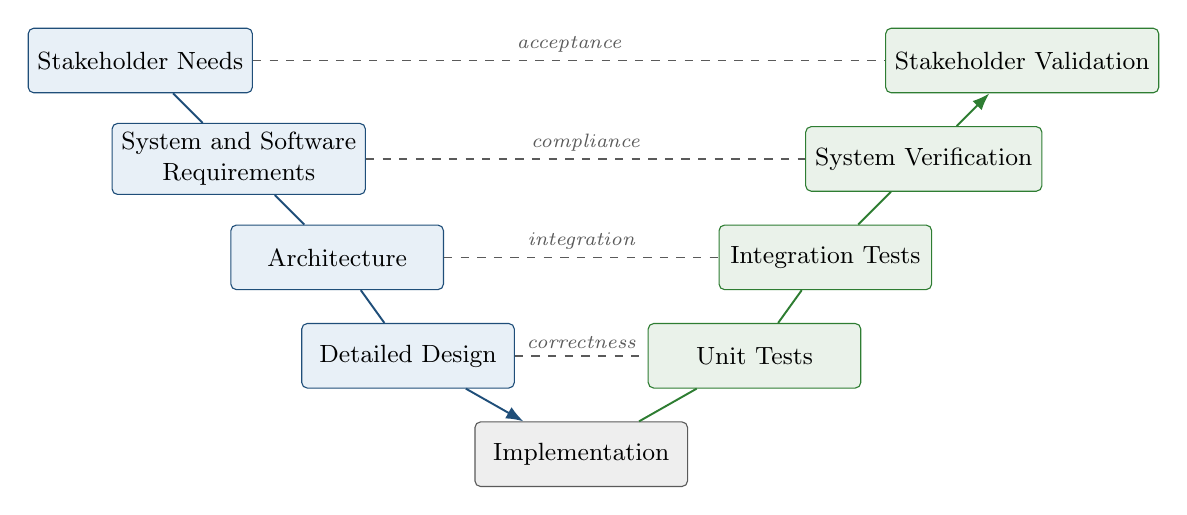
\begin{tikzpicture}[
  stage/.style={
    draw=dsnBlue,
    fill=dsnLightBlue,
    rounded corners=2pt,
    minimum width=2.7cm,
    minimum height=0.82cm,
    align=center,
    font=\small
  },
  test stage/.style={
    stage,
    draw=dsnGreen,
    fill=dsnGreen!10
  },
  implementation/.style={
    stage,
    draw=dsnGray,
    fill=dsnGray!10
  },
  lifecycle/.style={
    -{Latex[length=2.2mm]},
    line width=0.7pt
  },
  relationship/.style={
    draw=dsnGray,
    dashed,
    line width=0.6pt
  },
  relationship label/.style={
    fill=white,
    inner sep=1.5pt,
    font=\scriptsize\itshape,
    text=dsnGray
  }
]
  \node[stage] (needs) at (-5.6,5.0) {Stakeholder Needs};
  \node[stage, minimum width=3.2cm] (requirements) at (-4.35,3.75) {System and Software\\Requirements};
  \node[stage] (architecture) at (-3.1,2.5) {Architecture};
  \node[stage] (design) at (-2.2,1.25) {Detailed Design};
  \node[implementation] (implementation) at (0,0) {Implementation};

  \node[test stage] (unit) at (2.2,1.25) {Unit Tests};
  \node[test stage] (integration) at (3.1,2.5) {Integration Tests};
  \node[test stage, minimum width=3.0cm] (verification) at (4.35,3.75) {System Verification};
  \node[test stage, minimum width=2.9cm] (validation) at (5.6,5.0) {Stakeholder Validation};

  \draw[lifecycle, draw=dsnBlue]
    (needs) -- (requirements) -- (architecture) -- (design) -- (implementation);
  \draw[lifecycle, draw=dsnGreen]
    (implementation) -- (unit) -- (integration) -- (verification) -- (validation);

  \draw[relationship] (needs) -- node[relationship label, above=1pt] {acceptance} (validation);
  \draw[relationship] (requirements) -- node[relationship label, above=1pt] {compliance} (verification);
  \draw[relationship] (architecture) -- node[relationship label, above=1pt] {integration} (integration);
  \draw[relationship] (design) -- node[relationship label, above=1pt] {correctness} (unit);

\end{tikzpicture}

\caption{V-model relationships used by this specification.}
\label{Figure:VModel}
\end{figure}

\chapter{Development Plan}
\ChapterLabel{DevelopmentPlan}
\section{How to Use This Chapter}
Describe governance, roles, milestones, change control, and risks. Adapt the plan to the lifecycle the team will actually follow.

\section{Roles and Approval Authority}
\label{Section:DevelopmentPlanRoles}
Stel Angelidis is the document owner and the authorized approver for
\ProjectName. Other project roles are TBD.

\section{Domain Profile Selection}
\label{Section:DevelopmentPlanProfiles}
Record every domain tailoring profile considered during initialization. An
authorized human shall set each profile to Applicable, Not Applicable, or TBD
and record the rationale, decision owner, and date. A TBD profile remains in
the AI and human review context until resolved. When a profile is Applicable,
identify the lifecycle gates, roles, evidence, and reviews it adds to this
development plan.

\small
\begin{tabularx}{\linewidth}{L{3.5cm}L{2.7cm}Y}
\caption{Project Domain Profile Decisions\label{Table:ProjectDomainProfiles}}\\
\toprule
\textbf{Profile} & \textbf{Status} & \textbf{Rationale, Owner, and Date}\\
\midrule
\endfirsthead
\multicolumn{3}{l}{\small\itshape Project Domain Profile Decisions (continued)}\\
\toprule
\textbf{Profile} & \textbf{Status} & \textbf{Rationale, Owner, and Date}\\
\midrule
\endhead
\bottomrule
\endlastfoot
\hyperref[Chapter:EmbeddedSystemsProfile]{Embedded Systems} &
Applicable &
The system controls the physical opening and closing of a curtain.
Platform: microcontroller; bare metal or RTOS is TBD. Specific
microcontroller, board, and hardware revisions: TBD. Approved by Stel
Angelidis on October 14, 2026.\\
\textit{[Additional profile]} &
\textit{[Applicable / Not Applicable / TBD]} &
\textit{[Decision basis, authorized owner, and decision date]}\\
\end{tabularx}
\normalsize

\section{Example}
The product owner prioritizes outcomes; the architect owns significant design decisions; developers implement approved work; and the test lead retains evidence. Typical gates are needs reviewed, requirements baselined, architecture approved, evidence complete, and release approved. Example risk: an external service may be unavailable; define the failure response and test it before release.

\chapter{System Context}
\ChapterLabel{SystemContext}
\section{How to Use This Chapter}
Define the problem, stakeholders, system boundary, external actors and systems, assumptions, dependencies, and exclusions. Add a context diagram when it clarifies interactions.
\section{System Purpose}
\label{Section:SystemPurpose}
\ProjectName\ controls the opening and closing of a curtain. The current
decision is that a user commands the curtain through both a physical
controller and a phone application.

\section{Stakeholders}
\label{Section:Stakeholders}
\index{stakeholder}
The stakeholders are people who want a low-cost \gls{iot} curtain closer that
does not invade their privacy. Stel Angelidis is the authorized approver (see
\hyperref[Section:DevelopmentPlanRoles]{approval authority}).

\section{Stakeholder Constraints}
\label{Section:StakeholderConstraints}
\index{privacy}
\index{cost limit}
\index{microcontroller}
The following constraints were stated by the authorized approver on
October 14, 2026. They are inputs to the Requirements chapter and are not yet
formal requirements.

\begin{itemize}
\item \textbf{Privacy:} the system collects no data about individual
people, and it includes no cameras or microphones.
\item \textbf{Cost:} the components cost no more than USD~20.
\item \textbf{Platform:} the system runs on a microcontroller. All other
platform characteristics are TBD.
\end{itemize}

\section{Open Context Items}
\label{Section:OpenContextItems}
The following context is TBD and shall be resolved from project evidence and
authorized decisions before requirements are developed:

\begin{itemize}
\item the specific users, operators, installers, and maintainers, and any
stakeholder groups beyond those identified in
Section~\ref{Section:Stakeholders};
\item the basis of the USD~20 component-cost limit, including whether it
applies to the total of all components, which items count (for example the
motor, power supply, enclosure, and mounting hardware), the purchase quantity,
and the pricing date;
\item whether any non-personal operational data, such as curtain position or
schedules, may be stored or transmitted, and whether any cloud or
third-party service is acceptable;
\item the physical-controller and phone-application interfaces, including
how the phone application communicates with the system;
\item the system boundary, including the curtain mechanism, any actuator,
sensors, or power source, and any external network, phone, or cloud service;
\item the specific microcontroller, whether it runs bare-metal firmware or
an RTOS, the board, and hardware revisions (see
\ChapterRef{EmbeddedSystemsProfile});
\item the physical installation environment, constraints, and assumptions;
and
\item a context diagram, once the boundary and external actors are known.
\end{itemize}

\textit{Template pattern: [User role] needs to [achieve outcome] because
[current problem]. The system manages [owned capability]; [external system]
remains outside the boundary and provides [interface]. Record its owner, data
exchanged, and failure assumptions.}

\chapter{User Stories}
\ChapterLabel{UserStories}
\index{user story}
\index{acceptance criterion}
\section{How to Use This Chapter}
Capture stakeholder goals in accessible language. Stories express value and
acceptance intent; precise obligations belong in Requirements. Give each story
a stable ID, a priority, and links to one or more requirements that implement it.

\section{User Story Register}
\begin{tabularx}{\linewidth}{L{1.9cm}YL{1.8cm}L{3.4cm}}
\caption{User Story Register\label{Table:UserStories}}\\
\toprule
\textbf{ID} & \textbf{Story and Acceptance Criteria} & \textbf{Priority} & \textbf{Requirement(s)}\\
\midrule
\endfirsthead
\multicolumn{4}{l}{\small\itshape User Story Register (continued)}\\
\toprule
\textbf{ID} & \textbf{Story and Acceptance Criteria} & \textbf{Priority} & \textbf{Requirement(s)}\\
\midrule
\endhead
\midrule
\multicolumn{4}{r}{\small\itshape Continued on next page}\\
\endfoot
\bottomrule
\endlastfoot
\UserStoryID{US-001} & As a customer, I want to submit a service request so that the responsible team can act on it. Acceptance: valid data produces a unique request identifier on every supported client. & \gls{must} & \RequirementRef{REQ-F-001}, \RequirementRef{REQ-C-001}\\
\UserStoryID{US-002} & As a customer, I want to view my request status so that I understand its progress. Acceptance: the current status and most recent update appear within the specified response time, and the transition history is retained. & \gls{should} & \RequirementRef{REQ-F-002}, \RequirementRef{REQ-Q-001}, \RequirementRef{REQ-D-001}, \RequirementRef{REQ-C-001}\\
\UserStoryID{US-003} & As an operations analyst, I want to export request history so that I can perform approved analysis. Acceptance: an authorized actor prepares complete history within five minutes in the approved versioned format without changing source records. & \gls{would} & \RequirementRef{REQ-B-001}, \RequirementRef{REQ-F-003}, \RequirementRef{REQ-I-001}, \RequirementRef{REQ-S-001}, \RequirementRef{REQ-D-001}, \RequirementRef{REQ-C-001}\\
\end{tabularx}

\section{Review Rules}
Confirm that every story identifies a beneficiary, outcome, acceptance
criterion, priority, and at least one linked requirement. Maintain reciprocal
story links in the traceability register.

\chapter{Requirements}
\ChapterLabel{Requirements}
\index{requirement}
\index{requirement!implementation version}
\index{priority}

\section{How to Use This Chapter}
State singular, necessary, unambiguous, feasible, and verifiable obligations.
Every requirement shall have a stable ID, one priority, the version in which it
was implemented, at least one mapped use case, and at least one mapped test case.
Enter \NoVersion\ in \textbf{In Version} when no implementation version has
been assigned. Preserve IDs when wording or version assignments change.

Select the requirement categories that make the specification easier to review
and govern. Keep each requirement in one primary register and use traceability
links instead of copying the same requirement into multiple categories.

\section{Requirement Identifier Naming Convention}
\label{Section:RequirementIdentifierConvention}
\index{requirement!identifier convention}
\index{requirement!family code}
\index{requirement!scope qualifier}

Requirement identifiers use the following grammar:
\begin{verbatim}
REQ-[<scope>-]<family>-<sequence>
\end{verbatim}
The optional scope qualifier identifies a project-defined subsystem, product,
content type, or other governed area. Omit it for project-wide requirements.
The sequence is a three-digit, zero-padded number that is unique within the
exact scope and family combination. For example, \texttt{REQ-F-004} is the
fourth project-wide functional requirement, while
\texttt{REQ-API-Q-003} is the third quality requirement in a project-defined
\texttt{API} scope.

\small
\begin{tabularx}{\linewidth}{L{2.0cm}L{3.5cm}Y}
\caption{Requirement Identifier Segments and Family Codes\label{Table:RequirementIdentifierConvention}}\\
\toprule
\textbf{Code} & \textbf{Meaning} & \textbf{Use}\\
\midrule
\endfirsthead
\multicolumn{3}{l}{\small\itshape Requirement Identifier Segments and Family Codes (continued)}\\
\toprule
\textbf{Code} & \textbf{Meaning} & \textbf{Use}\\
\midrule
\endhead
\bottomrule
\endlastfoot
\texttt{REQ} & Requirement & Identifies the artifact as a requirement. Every requirement ID begins with this segment.\\
\texttt{<scope>} & Project-defined scope & Optional uppercase qualifier for a governed subsystem, product, content type, or other area. Define every scope code before use; absence denotes project-wide scope.\\
\texttt{B} & Business & States the stakeholder outcome, mission, commercial purpose, policy goal, or business result the system shall enable.\\
\texttt{F} & Functional & States observable behavior, service, workflow, calculation, state change, or capability the system shall provide.\\
\texttt{Q} & Quality & States a measurable quality attribute or non-functional expectation, including accessibility, performance, reliability, resilience, usability, maintainability, or compatibility.\\
\texttt{I} & Interface & States a user, software, API, hardware, communication, protocol, or external-system boundary contract, including integration behavior at that boundary.\\
\texttt{S} & Security & States security, privacy, consent, authorization, auditing, secret-handling, or protected-data obligations maintained in a specialized security register.\\
\texttt{D} & Data & States data definition, authority, provenance, quality, integrity, ownership, lifecycle, retention, or source-of-truth obligations.\\
\texttt{C} & Constraint & States a binding implementation, platform, technology, format, storage, source-control, standards, compatibility, schedule, budget, or governance constraint.\\
\texttt{\#\#\#} & Sequence & Three-digit, zero-padded stable sequence within the exact scope and family; assigned monotonically and never reused.\\
\bottomrule
\end{tabularx}
\normalsize

Classify a requirement by its primary obligation and verification concern. A
requirement may support several concerns, but its identifier contains only one
family code. Represent cross-cutting relationships through traceability rather
than a compound family code.

An AI agent shall reuse an existing scope and family whenever their definitions
fit. If no defined family accurately represents the requirement, the agent
shall not silently invent or use a new code. It shall propose a unique uppercase
code, full family name, decision boundary, rationale, and representative
examples; check the complete requirements register and category catalog for
semantic overlap and identifier collision; and obtain authorized-human
approval. After approval, the agent shall add the family to
Table~\ref{Table:RequirementIdentifierConvention}, update the category catalog
and AI guidance, and create or update the applicable register before assigning
an identifier from it. The same approval and documentation rule applies to a
new scope qualifier. Extending the convention shall not rename, renumber, or
reuse an existing identifier.

\section{Functional and Quality Requirements}
\index{requirement!functional}
\index{requirement!quality}
Functional and quality requirements answer different questions and shall not be
used interchangeably.

\begin{dsnNote}[Central Distinction]
A \textbf{functional requirement} states what behavior, service, calculation,
state transition, or externally observable result the system shall provide. A
\textbf{quality requirement} states how well that behavior or the system as a
whole shall perform under stated conditions. Quality requirements require a
measurable threshold, workload, environment, or other evaluation basis.
\end{dsnNote}

For example, ``The system shall display the current request status'' is
functional. ``The system shall display the current request status within two
seconds under the reference workload'' is a quality requirement. Avoid vague
quality statements such as ``the system shall be fast, secure, reliable, or
easy to use.'' Replace them with measurable conditions and success criteria.

Quality requirements are also called quality-attribute or non-functional
requirements. The term \emph{quality requirement} is preferred here because
these obligations describe behavior that shall be designed, implemented, and
verified rather than an absence of function.

\section{Requirement Status Model}
\index{requirement!status}
\index{status!Open}
\index{status!In Progress}
\index{status!Done}
\index{status!Retired}
Priority and status are independent. Priority records the requirement's
importance or commitment; status records its progress through the delivery
lifecycle. A status change shall not erase or replace the assigned priority.

\begin{tabularx}{\linewidth}{L{3.0cm}YL{3.3cm}}
\caption{Requirement Status Definitions\label{Table:RequirementStatusDefinitions}}\\
\toprule
\textbf{Status} & \textbf{Meaning} & \textbf{In Version Rule}\\
\midrule
\endfirsthead
\toprule
\textbf{Status} & \textbf{Meaning} & \textbf{In Version Rule}\\
\midrule
\endhead
\ReqStatusOpen & The requirement is active, but implementation has not started. Deferred work remains Open until work begins or the requirement is retired. & Enter \NoVersion.\\
\ReqStatusInProgress & Implementation or integration work has started, but the requirement does not yet satisfy the definition of Done. & Enter \NoVersion.\\
\ReqStatusDone & The requirement is implemented; mapped tests pass; verification is complete; traceability is current; and the completed behavior is included in a controlled version. & Enter the first controlled version containing the completed requirement.\\
\ReqStatusRetired & The requirement is no longer active because it was superseded, made obsolete, rejected, or withdrawn. Retain its stable ID, original text, and traceability; record the rationale and any replacement in document history. & Retain the original implementation version if it was previously Done; otherwise enter \NoVersion.\\
\bottomrule
\end{tabularx}

Only \ReqStatusDone\ asserts completion. Do not remove a retired requirement or
reuse its ID. A requirement may move from \ReqStatusRetired\ only through an
approved change that restores its active status and records the decision in
document history.

\section{Requirement Category Catalog}
\index{requirement!category catalog}
The following catalog distinguishes broad requirement families from their
subtypes. In particular, performance, capacity, scalability, reliability,
availability, resilience, recoverability, usability, accessibility,
maintainability, supportability, testability, portability, compatibility,
interoperability, security, privacy, safety, sustainability, and observability
are quality attributes. A requirement concerning one of these attributes is a
quality requirement when it specifies how well the system shall operate under
stated conditions.

A project may organize a specialized quality attribute, such as security,
privacy, or safety, in a separate register when it has distinct owners, review
criteria, evidence, or assurance obligations. The separate register is a
management view; it does not change the requirement's classification as a
quality requirement. Likewise, interface, data, operational, and other families
may contain both functional obligations and associated quality obligations. Use
the primary purpose of each requirement to select its register and use links to
represent cross-cutting concerns.

The catalog is intentionally broad. A project may use a family as a top-level
register, create registers for selected subtypes, combine closely related
groups, or omit groups that do not apply. Category choice shall not weaken the
traceability or verification rules for individual requirements.

\section{Domain Profile Impact on Requirements}
\label{Section:DomainProfileRequirements}
\index{requirement!domain profile}
Every Applicable domain profile shall be evaluated when developing or changing
requirements. Each applicable profile concern shall result in one or more
project requirements, a reference to an existing requirement, or a documented
Not Applicable decision with rationale approved by an authorized human. Record
the profile applicability decision in the Development Plan and retain
project-specific obligations only in the applicable requirement registers.
The profile itself is a tailoring guide, not a duplicate requirements
specification. See Section~\ref{Section:DomainProfiles} and the applicable
profile appendix.

\small
\begin{tabularx}{\linewidth}{L{3.0cm}L{4.0cm}Y}
\caption{Requirement Families, Subtypes, and Quality Attributes\label{Table:RequirementCategoryCatalog}}\\
\toprule
\textbf{Requirement Family} & \textbf{Subtype or Quality Attribute} & \textbf{Typical Scope}\\
\midrule
\endfirsthead
\multicolumn{3}{l}{\small\itshape Requirement Families, Subtypes, and Quality Attributes (continued)}\\
\toprule
\textbf{Requirement Family} & \textbf{Subtype or Quality Attribute} & \textbf{Typical Scope}\\
\midrule
\endhead
\midrule
\multicolumn{3}{r}{\small\itshape Continued on next page}\\
\endfoot
\bottomrule
\endlastfoot
Business & Outcomes and policy & Organizational outcomes, value, policy goals, measurable benefits, cost targets, and mission objectives.\\
Stakeholder and user & Stakeholder need & Capabilities, outcomes, and constraints needed by a stakeholder group or external party.\\
Stakeholder and user & User need & User goals and externally visible outcomes expressed independently of a particular implementation.\\
Functional & System behavior & Services, calculations, decisions, state changes, workflows, and observable system responses.\\
Quality & General quality & Measurable characteristics that state how well a function or the system shall operate under stated conditions.\\
Quality & Performance & Response time, latency, throughput, processing time, and resource consumption.\\
Quality & Capacity & Supported data volume, transaction volume, concurrent users, devices, or retained records.\\
Quality & Scalability & Behavior as workload, data, users, or deployed instances increase or decrease.\\
Quality & Reliability & Probability or frequency of failure-free operation under stated conditions.\\
Quality & Availability & Required service availability, planned downtime, and permitted outage duration.\\
Quality & Resilience and fault tolerance & Continued or degraded operation when components, dependencies, or communication paths fail.\\
Quality & Recoverability and continuity & Recovery time, recovery point, restoration, backup, failover, and disaster-continuity objectives.\\
Quality & Usability & Task effectiveness, efficiency, learnability, error prevention, and user satisfaction.\\
Quality & Accessibility & Conformance and measurable support for users with visual, auditory, motor, speech, or cognitive disabilities.\\
Quality & Maintainability & Time, effort, modularity, analyzability, and change characteristics required for system modification.\\
Quality & Supportability & Diagnostic access, service procedures, field replacement, support hours, and support-team capabilities.\\
Quality & Testability & Controllability, observability, repeatability, test interfaces, and evidence needed to verify behavior.\\
Quality & Portability & Ability to install, move, or operate the system across specified environments or platforms.\\
Quality & Compatibility & Coexistence and correct operation with specified versions, devices, browsers, operating systems, or products.\\
Quality & Interoperability & Coordinated behavior, protocols, semantics, orchestration, and exchanges with external systems.\\
Quality & Security & Authentication, authorization, confidentiality, integrity, cryptography, auditing, and threat resistance.\\
Quality & Privacy & Collection, consent, purpose, minimization, access, disclosure, retention, deletion, and rights for personal data.\\
Quality & Safety & Hazard prevention, risk reduction, safe state, interlocks, alarms, and unacceptable-loss controls.\\
Quality & Sustainability & Energy use, resource efficiency, carbon reporting, hardware life, repair, reuse, and disposal objectives.\\
Quality & Observability & Logs, metrics, traces, health signals, diagnostic context, and measurable diagnostic coverage.\\
Interface & User interface & Human-system interaction, presentation, navigation, input, feedback, and interaction contracts.\\
Interface & Software and API & Operations, messages, schemas, errors, protocols, sequencing, and software boundary contracts.\\
Interface & Hardware and communication & Connectors, signals, electrical characteristics, device protocols, networks, and physical boundaries.\\
Data and information & Data definition and quality & Data definitions, schemas, provenance, accuracy, completeness, integrity, ownership, and permitted transformations.\\
Data and information & Lifecycle and governance & Creation, access, retention, archival, legal hold, disposition, deletion, and proof of destruction.\\
Operational & Operation and administration & Startup, shutdown, scheduling, configuration, provisioning, monitoring, backup, recovery, and incident response.\\
Operational & Deployment and platform & Approved platforms, topology, packaging, installation, configuration, upgrade, and runtime environment.\\
Operational & Infrastructure and environment & Network, compute, storage, facility, power, temperature, physical location, and environmental limits.\\
Transition & Migration and rollout & Data conversion, coexistence, rollout, cutover, rollback, legacy integration, and decommissioning.\\
Compliance and legal & Regulatory and standards & Obligations imposed by regulations, standards, certifications, policies, or assurance frameworks.\\
Compliance and legal & Legal and contractual & Licenses, warranties, intellectual-property terms, service agreements, procurement terms, and contractual duties.\\
Compliance and legal & Reporting and audit & Reports, evidence, audit trails, review access, content, timing, and record accountability.\\
Product support & Documentation & Required user, operator, administrator, developer, API, maintenance, and compliance documentation.\\
Product support & Training & Required curricula, exercises, qualifications, delivery modes, and demonstrated learner outcomes.\\
Commercial & Licensing and entitlement & Product editions, entitlement, metering, third-party components, subscriptions, and licensing restrictions.\\
AI and machine learning & Model and data controls & Model performance, data provenance, bias evaluation, explainability, human oversight, drift, and retraining controls.\\
Physical and hardware & Physical characteristics & Dimensions, mass, materials, connectors, tolerances, environmental ratings, and hardware behavior.\\
Constraint & Solution constraint & Mandated technologies, designs, budgets, schedules, standards, dependencies, or solution boundaries.\\
\end{tabularx}
\normalsize

\section{Creating a Project-Specific Category}
Create an additional category when it gives requirements a distinct meaning,
owner, review method, or assurance process. Define the category's scope and a
unique family code using
Section~\ref{Section:RequirementIdentifierConvention}; duplicate one of the
category-specific registers below; keep the standard columns; add the category to
\hyperref[Table:RequirementCategoryCatalog]{the category catalog}; and update
use cases, tests, traceability, verification, validation, document history, and
the index as applicable. Document whether the new category is top-level or a
subtype of an existing category.

Do not create a category solely to avoid resolving an ambiguous requirement.
If one statement contains multiple independently verifiable obligations, split
it into singular requirements and assign each one a primary category.

\section{Review Rules}
Reject a requirement row if its priority, status, use-case mapping, or test-case
mapping is empty. The \textbf{Status} field shall contain Open, In Progress,
Done, or Retired. The \textbf{In Version} field shall follow
\hyperref[Table:RequirementStatusDefinitions]{the status definitions}. Confirm
that reciprocal mappings appear in the user-story, use-case, test,
traceability, and verification registers.

\begin{landscape}
\small
\section{Category-Specific Requirement Registers}
The seven registers below are the template's default working set. They are
selected for practical review and ownership, not as seven mutually exclusive
top-level families. For example, the Security Requirements Register is a
specialized quality-requirement register. Add, rename, combine, or remove
registers to match the approved project taxonomy. Every retained register shall
use the same traceability columns.

\subsection{Business Requirements}
\index{requirement!business}
\begin{tabularx}{\linewidth}{L{2.1cm}YL{2.0cm}L{2.1cm}L{1.5cm}L{2.6cm}L{2.6cm}}
\caption{Business Requirements Register\label{Table:BusinessRequirements}}\\
\toprule
\textbf{ID} & \textbf{Requirement} & \textbf{Priority} & \textbf{Status} & \textbf{In Version} & \textbf{Use Case(s)} & \textbf{Test Case(s)}\\
\midrule
\endfirsthead
\multicolumn{7}{l}{\small\itshape Business Requirements Register (continued)}\\
\toprule
\textbf{ID} & \textbf{Requirement} & \textbf{Priority} & \textbf{Status} & \textbf{In Version} & \textbf{Use Case(s)} & \textbf{Test Case(s)}\\
\midrule
\endhead
\midrule
\multicolumn{7}{r}{\small\itshape Continued on next page}\\
\endfoot
\bottomrule
\endlastfoot
\RequirementID{REQ-B-001} & The system shall enable an authorized analyst to prepare approved request-history data for analysis within five minutes for the reference data set. & \gls{must} & \ReqStatusOpen & \NoVersion & \UseCaseRef{UC-003} & \TestCaseRef{TC-009}\\
\end{tabularx}

\clearpage
\subsection{Functional Requirements}
\begin{tabularx}{\linewidth}{L{2.1cm}YL{2.0cm}L{2.1cm}L{1.5cm}L{2.6cm}L{2.6cm}}
\caption{Functional Requirements Register\label{Table:FunctionalRequirements}}\\
\toprule
\textbf{ID} & \textbf{Requirement} & \textbf{Priority} & \textbf{Status} & \textbf{In Version} & \textbf{Use Case(s)} & \textbf{Test Case(s)}\\
\midrule
\endfirsthead
\multicolumn{7}{l}{\small\itshape Functional Requirements Register (continued)}\\
\toprule
\textbf{ID} & \textbf{Requirement} & \textbf{Priority} & \textbf{Status} & \textbf{In Version} & \textbf{Use Case(s)} & \textbf{Test Case(s)}\\
\midrule
\endhead
\midrule
\multicolumn{7}{r}{\small\itshape Continued on next page}\\
\endfoot
\bottomrule
\endlastfoot
\RequirementID{REQ-F-001} & The system shall accept a valid service request and assign it a unique identifier. & \gls{must} & \ReqStatusDone & 1.0 & \UseCaseRef{UC-001} & \TestCaseRef{TC-001}\\
\RequirementID{REQ-F-002} & The system shall display the current status and most recent update for a submitted request. & \gls{should} & \ReqStatusDone & 1.1 & \UseCaseRef{UC-002} & \TestCaseRef{TC-002}\\
\RequirementID{REQ-F-003} & The system shall export request history in the approved interchange format. & \gls{would} & \ReqStatusOpen & \NoVersion & \UseCaseRef{UC-003} & \TestCaseRef{TC-004}\\
\end{tabularx}

\subsection{Quality Requirements}
\begin{tabularx}{\linewidth}{L{2.1cm}YL{2.0cm}L{2.1cm}L{1.5cm}L{2.6cm}L{2.6cm}}
\caption{Quality Requirements Register\label{Table:QualityRequirements}}\\
\toprule
\textbf{ID} & \textbf{Requirement} & \textbf{Priority} & \textbf{Status} & \textbf{In Version} & \textbf{Use Case(s)} & \textbf{Test Case(s)}\\
\midrule
\endfirsthead
\multicolumn{7}{l}{\small\itshape Quality Requirements Register (continued)}\\
\toprule
\textbf{ID} & \textbf{Requirement} & \textbf{Priority} & \textbf{Status} & \textbf{In Version} & \textbf{Use Case(s)} & \textbf{Test Case(s)}\\
\midrule
\endhead
\midrule
\multicolumn{7}{r}{\small\itshape Continued on next page}\\
\endfoot
\bottomrule
\endlastfoot
\RequirementID{REQ-Q-001} & The system shall display a request status within two seconds under the reference workload. & \gls{could} & \ReqStatusDone & 1.2 & \UseCaseRef{UC-002} & \TestCaseRef{TC-003}\\
\end{tabularx}

\clearpage
\subsection{Interface Requirements}
\index{requirement!interface}
\begin{tabularx}{\linewidth}{L{2.1cm}YL{2.0cm}L{2.1cm}L{1.5cm}L{2.6cm}L{2.6cm}}
\caption{Interface Requirements Register\label{Table:InterfaceRequirements}}\\
\toprule
\textbf{ID} & \textbf{Requirement} & \textbf{Priority} & \textbf{Status} & \textbf{In Version} & \textbf{Use Case(s)} & \textbf{Test Case(s)}\\
\midrule
\endfirsthead
\multicolumn{7}{l}{\small\itshape Interface Requirements Register (continued)}\\
\toprule
\textbf{ID} & \textbf{Requirement} & \textbf{Priority} & \textbf{Status} & \textbf{In Version} & \textbf{Use Case(s)} & \textbf{Test Case(s)}\\
\midrule
\endhead
\midrule
\multicolumn{7}{r}{\small\itshape Continued on next page}\\
\endfoot
\bottomrule
\endlastfoot
\RequirementID{REQ-I-001} & The system shall exchange request-history exports using the approved, versioned interface schema. & \gls{should} & \ReqStatusInProgress & \NoVersion & \UseCaseRef{UC-003} & \TestCaseRef{TC-005}\\
\end{tabularx}

\subsection{Security Requirements}
\index{requirement!security}
\begin{tabularx}{\linewidth}{L{2.1cm}YL{2.0cm}L{2.1cm}L{1.5cm}L{2.6cm}L{2.6cm}}
\caption{Security Requirements Register\label{Table:SecurityRequirements}}\\
\toprule
\textbf{ID} & \textbf{Requirement} & \textbf{Priority} & \textbf{Status} & \textbf{In Version} & \textbf{Use Case(s)} & \textbf{Test Case(s)}\\
\midrule
\endfirsthead
\multicolumn{7}{l}{\small\itshape Security Requirements Register (continued)}\\
\toprule
\textbf{ID} & \textbf{Requirement} & \textbf{Priority} & \textbf{Status} & \textbf{In Version} & \textbf{Use Case(s)} & \textbf{Test Case(s)}\\
\midrule
\endhead
\midrule
\multicolumn{7}{r}{\small\itshape Continued on next page}\\
\endfoot
\bottomrule
\endlastfoot
\RequirementID{REQ-S-001} & The system shall permit request-history exports only to authenticated actors assigned the approved export role. & \gls{must} & \ReqStatusDone & 1.0 & \UseCaseRef{UC-003} & \TestCaseRef{TC-006}\\
\end{tabularx}

\clearpage
\subsection{Data Requirements}
\index{requirement!data}
\begin{tabularx}{\linewidth}{L{2.1cm}YL{2.0cm}L{2.1cm}L{1.5cm}L{2.6cm}L{2.6cm}}
\caption{Data Requirements Register\label{Table:DataRequirements}}\\
\toprule
\textbf{ID} & \textbf{Requirement} & \textbf{Priority} & \textbf{Status} & \textbf{In Version} & \textbf{Use Case(s)} & \textbf{Test Case(s)}\\
\midrule
\endfirsthead
\multicolumn{7}{l}{\small\itshape Data Requirements Register (continued)}\\
\toprule
\textbf{ID} & \textbf{Requirement} & \textbf{Priority} & \textbf{Status} & \textbf{In Version} & \textbf{Use Case(s)} & \textbf{Test Case(s)}\\
\midrule
\endhead
\midrule
\multicolumn{7}{r}{\small\itshape Continued on next page}\\
\endfoot
\bottomrule
\endlastfoot
\RequirementID{REQ-D-001} & The system shall retain each request status transition with its timestamp, actor identifier, previous status, and new status. & \gls{must} & \ReqStatusDone & 1.1 & \UseCaseRef{UC-002}, \UseCaseRef{UC-003} & \TestCaseRef{TC-007}\\
\end{tabularx}

\subsection{Constraint Requirements}
\index{requirement!constraint}
\begin{tabularx}{\linewidth}{L{2.1cm}YL{2.0cm}L{2.1cm}L{1.5cm}L{2.6cm}L{2.6cm}}
\caption{Constraint Requirements Register\label{Table:ConstraintRequirements}}\\
\toprule
\textbf{ID} & \textbf{Requirement} & \textbf{Priority} & \textbf{Status} & \textbf{In Version} & \textbf{Use Case(s)} & \textbf{Test Case(s)}\\
\midrule
\endfirsthead
\multicolumn{7}{l}{\small\itshape Constraint Requirements Register (continued)}\\
\toprule
\textbf{ID} & \textbf{Requirement} & \textbf{Priority} & \textbf{Status} & \textbf{In Version} & \textbf{Use Case(s)} & \textbf{Test Case(s)}\\
\midrule
\endhead
\midrule
\multicolumn{7}{r}{\small\itshape Continued on next page}\\
\endfoot
\bottomrule
\endlastfoot
\RequirementID{REQ-C-001} & The system shall support the deployment platform and browser versions identified in the approved deployment baseline. & \gls{must} & \ReqStatusDone & 1.0 & \UseCaseRef{UC-001}, \UseCaseRef{UC-002}, \UseCaseRef{UC-003} & \TestCaseRef{TC-008}\\
\end{tabularx}
\end{landscape}

\chapter{Use Cases}
\ChapterLabel{UseCases}
\section{How to Use This Chapter}
Describe goal-oriented interactions at the system boundary. Give every use case
a stable ID, its own table, and at least one reciprocal requirement mapping.
Include preconditions, trigger, main flow, alternate or exception flows, and
postconditions. Maintain the canonical relationships among stories,
requirements, use cases, and tests in \ChapterRef{Traceability}.

\section[High-Level Use Case Diagram]{\hspace{0.5em}High-Level Use Case Diagram}
Show the system boundary, primary actors, and major user goals before the
detailed use-case tables. Replace the generic example with project-specific
actors and use cases while preserving the stable use-case identifiers.
Figure~\ref{Figure:UseCaseDiagram} provides the template example.

\begin{figure}[htbp]
\centering
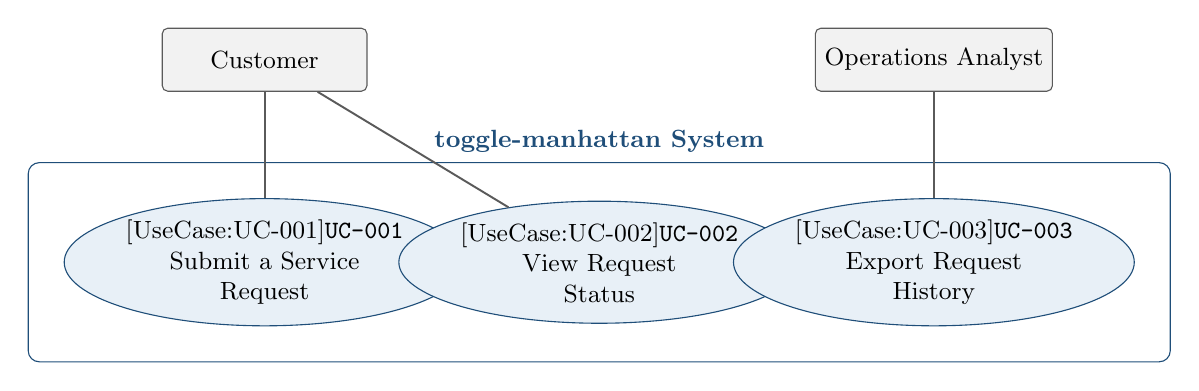
\begin{tikzpicture}[
  actor/.style={
    draw=dsnGray,
    fill=dsnGray!8,
    rounded corners=2pt,
    minimum width=2.6cm,
    minimum height=0.8cm,
    align=center,
    font=\small
  },
  use case/.style={
    ellipse,
    draw=dsnBlue,
    fill=dsnLightBlue,
    minimum width=3.8cm,
    minimum height=1.55cm,
    inner sep=1pt,
    align=center,
    font=\small
  },
  association/.style={
    draw=dsnGray,
    line width=0.7pt
  },
  system boundary/.style={
    draw=dsnBlue,
    rounded corners=4pt,
    inner sep=0.45cm
  }
]
  \node[use case] (submit) at (0,0) {\UseCaseRef{UC-001}\\Submit a Service\\Request};
  \node[use case] (status) at (4.25,0) {\UseCaseRef{UC-002}\\View Request\\Status};
  \node[use case] (export) at (8.5,0) {\UseCaseRef{UC-003}\\Export Request\\History};

  \node[system boundary, fit=(submit)(status)(export),
    label={[font=\small\bfseries, text=dsnBlue]above:\ProjectName\ System}]
    (system) {};

  \node[actor, above=1.35cm of submit] (customer) {Customer};
  \node[actor, above=1.35cm of export] (analyst) {Operations Analyst};

  \draw[association] (customer) -- (submit);
  \draw[association] (customer) -- (status);
  \draw[association] (analyst) -- (export);
\end{tikzpicture}

\caption{Generic high-level use case diagram.}
\label{Figure:UseCaseDiagram}
\end{figure}
\index{use case diagram}

\section{Submit a Service Request}
\begin{tabularx}{\linewidth}{L{3.5cm}Y}
\toprule
\textbf{Identifier} & \UseCaseID{UC-001}\\
\textbf{Mapped requirements} & \RequirementRef{REQ-F-001}, \RequirementRef{REQ-C-001}\\
\textbf{Goal} & Submit a valid request and receive a unique identifier.\\
\textbf{Primary actor} & Customer\\
\textbf{Preconditions} & The customer can access the request form.\\
\textbf{Trigger} & The customer chooses to submit a new request.\\
\textbf{Main flow} & The customer enters required data and submits it; the system validates the data, creates the request, and displays its identifier.\\
\textbf{Alternate flow} & If required data is invalid, the system identifies the affected fields and creates no request.\\
\textbf{Postconditions} & A valid request exists with a unique identifier and an initial status.\\
\bottomrule
\end{tabularx}

\section{View Request Status}
\begin{tabularx}{\linewidth}{L{3.5cm}Y}
\toprule
\textbf{Identifier} & \UseCaseID{UC-002}\\
\textbf{Mapped requirements} & \RequirementRef{REQ-F-002}, \RequirementRef{REQ-Q-001}, \RequirementRef{REQ-D-001}, \RequirementRef{REQ-C-001}\\
\textbf{Goal} & Review the current state of a submitted request.\\
\textbf{Primary actor} & Customer\\
\textbf{Preconditions} & A request with a known identifier exists.\\
\textbf{Trigger} & The customer opens or refreshes the request status.\\
\textbf{Main flow} & The system retrieves and displays the request status and most recent update.\\
\textbf{Alternate flow} & If the identifier is unknown, the system reports that no matching request was found.\\
\textbf{Postconditions} & The request remains unchanged; its current status has been presented.\\
\bottomrule
\end{tabularx}

\section{Export Request History}
\begin{tabularx}{\linewidth}{L{3.5cm}Y}
\toprule
\textbf{Identifier} & \UseCaseID{UC-003}\\
\textbf{Mapped requirements} & \RequirementRef{REQ-B-001}, \RequirementRef{REQ-F-003}, \RequirementRef{REQ-I-001}, \RequirementRef{REQ-S-001}, \RequirementRef{REQ-D-001}, \RequirementRef{REQ-C-001}\\
\textbf{Goal} & Export request history for authorized analysis.\\
\textbf{Primary actor} & Operations analyst\\
\textbf{Preconditions} & The actor is authorized and matching requests exist.\\
\textbf{Trigger} & The actor selects an export range and format.\\
\textbf{Main flow} & The system validates authorization, generates the export, and makes the result available to the actor.\\
\textbf{Alternate flow} & If no records match, the system produces an empty result with an explanatory status.\\
\textbf{Postconditions} & An export artifact exists; source request records are unchanged.\\
\bottomrule
\end{tabularx}

\chapter{Architecture Overview}
\ChapterLabel{ArchitectureOverview}
\section{How to Use This Chapter}
Explain the forces that shape the design, the major decisions, alternatives considered, and consequences. Use the 4+1 views only when they help readers answer different architectural questions.
\section{Decision Template and Example}
\textbf{ARC-001:} \textit{[Decision]}; \textbf{Drivers:} \textit{[quality attributes and constraints]}; \textbf{Rationale:} \textit{[why selected]}; \textbf{Consequences:} \textit{[benefits, trade-offs, and risks]}. Example: use an asynchronous message queue to protect request processing from transient downstream outages; this improves resilience but introduces eventual consistency.

\chapter{User Interface Design}
\ChapterLabel{UserInterfaceDesign}
\section{How to Use This Chapter}
Describe personas, primary screens or workflows, interaction rules, feedback, accessibility, and essential states. Include wireframes or prototypes where they resolve meaningful ambiguity.
\section{Example}
Persona: a busy operations coordinator needs to submit and track requests quickly. The request screen groups required fields, identifies inline validation errors, confirms successful submission, supports keyboard operation, and exposes empty, loading, error, and completed states.

\chapter{Logical View}
\ChapterLabel{LogicalView}
\section{How to Use This Chapter}
Model the domain concepts, responsibilities, relationships, data ownership, and invariants without committing to code-level structure. Use a class, entity, or conceptual diagram where useful.
\section{Example}
\textit{Request} has an identifier, submitter, status, and submitted time. A request has one or more \textit{Request Items}. Invariants: every identifier is unique; every request has a valid status; an approved request cannot return to Draft without an authorized transition.

\chapter{Process View}
\ChapterLabel{ProcessView}
\section{How to Use This Chapter}
Describe runtime behavior, concurrency, state transitions, workflows, error handling, and significant sequences. Use activity, sequence, or state diagrams when prose is insufficient.
\section{Example State Model}
Request states are Draft, Submitted, Under Review, Approved, Rejected, and Cancelled. Submission moves Draft to Submitted only when required data is valid. Approval and rejection are terminal except for an authorized correction workflow.

\chapter{Development View}
\ChapterLabel{DevelopmentView}
\section{How to Use This Chapter}
Show how source code, modules, services, libraries, and build artifacts are organized. State dependency rules so that implementers do not create forbidden coupling.
\section{Example}
Organize a service into presentation/API, application workflow, domain model, and infrastructure adapters. The API calls application services; application services depend on domain abstractions; infrastructure implements those abstractions. Domain logic must not depend on the web framework or database driver.

\chapter{Physical View}
\ChapterLabel{PhysicalView}
\section{How to Use This Chapter}
Describe deployment nodes, networks, environments, runtime dependencies, trust boundaries, data stores, and operations constraints. Include a deployment diagram for distributed systems.
\section{Example}
A browser communicates over TLS with an API service. The API service uses a private database network; backups are encrypted and access is limited to the operations role. Define availability targets, monitoring, and recovery responsibilities.

\chapter{Implementation}
\ChapterLabel{Implementation}
\section{How to Use This Chapter}
Document the selected technology baseline, build and run instructions, coding conventions that enforce architecture, configuration, and definition of done. Keep design rationale in Architecture Overview.
\section{Example}
The implementation uses [language], [framework], and [database]. Build with \texttt{[command]}; run with \texttt{[command]}. Configuration comes from [approved source]; credentials are never stored in source control. Completion requires passing tests, reviewed traceability, and approved evidence.

\chapter{Tests}
\ChapterLabel{Tests}
\section{How to Use This Chapter}
Define repeatable test cases, levels, environments, data, entry conditions, procedures, expected results, and result recording. Tests produce evidence; they do not replace verification or validation.
\section{Example Test Cases}
\begin{tabularx}{\linewidth}{L{2.1cm}L{3.0cm}YL{5.0cm}}
\caption{Test Case Examples\label{Table:TestCaseExamples}}\\
\toprule
\textbf{ID} & \textbf{Mapped Requirement} & \textbf{Procedure} & \textbf{Expected Result}\\
\midrule
\endfirsthead
\toprule
\textbf{ID} & \textbf{Mapped Requirement} & \textbf{Procedure} & \textbf{Expected Result}\\
\midrule
\endhead
\TestCaseID{TC-001} & \RequirementRef{REQ-F-001} & Submit a request containing valid required data. & The system creates one request and displays a unique identifier.\\
\TestCaseID{TC-002} & \RequirementRef{REQ-F-002} & Open the status for a known request. & The current status and most recent update are displayed.\\
\TestCaseID{TC-003} & \RequirementRef{REQ-Q-001} & Measure 20 status requests under the reference workload. & Every measured response is displayed within two seconds.\\
\TestCaseID{TC-004} & \RequirementRef{REQ-F-003} & Export a known request set in the approved format. & The export contains the expected history without changing source records.\\
\TestCaseID{TC-005} & \RequirementRef{REQ-I-001} & Export representative request history and validate the result against the approved interface schema version. & The export conforms to the approved schema and declares the expected schema version.\\
\TestCaseID{TC-006} & \RequirementRef{REQ-S-001} & Attempt the same export as an authorized actor, an authenticated actor without the export role, and an unauthenticated actor. & Only the authorized actor receives an export; both unauthorized attempts are denied and recorded.\\
\TestCaseID{TC-007} & \RequirementRef{REQ-D-001} & Perform two status transitions and inspect the stored history and exported record. & Each transition retains the expected timestamp, actor identifier, previous status, and new status.\\
\TestCaseID{TC-008} & \RequirementRef{REQ-C-001} & Execute the critical use-case test suite on every platform and browser version in the approved deployment baseline. & Every critical use case passes on every approved platform and browser version.\\
\TestCaseID{TC-009} & \RequirementRef{REQ-B-001} & Time an authorized analyst preparing an approved export from the reference data set without manual reconstruction. & The analyst obtains analysis-ready request-history data within five minutes.\\
\bottomrule
\end{tabularx}

\chapter{Traceability}
\ChapterLabel{Traceability}
\index{traceability}
\index{requirements traceability matrix}
\section{How to Use This Chapter}
Maintain the canonical mapping from stakeholder need or approved constraint through requirement, design decision, implementation, test, verification, validation, and release evidence. Review both missing backward links and missing forward links.
\section{Traceability Register}
Requirement and use-case chapters shall contain reciprocal mappings. An
unlinked requirement may be gold-plating; an untested requirement or unmapped
use case is incomplete.

\begin{landscape}
\small
\begin{tabularx}{\linewidth}{YYYYYY}
\caption{Traceability Register\label{Table:TraceabilityMatrix}}\\
\toprule
\textbf{User Story} & \textbf{Requirement} & \textbf{Use Case} & \textbf{Test Case} & \textbf{Verification} & \textbf{Validation}\\
\midrule
\endfirsthead
\multicolumn{6}{l}{\small\itshape Traceability Register (continued)}\\
\toprule
\textbf{User Story} & \textbf{Requirement} & \textbf{Use Case} & \textbf{Test Case} & \textbf{Verification} & \textbf{Validation}\\
\midrule
\endhead
\midrule
\multicolumn{6}{r}{\small\itshape Continued on next page}\\
\endfoot
\bottomrule
\endlastfoot
\UserStoryRef{US-001} & \RequirementRef{REQ-F-001} & \UseCaseRef{UC-001} & \TestCaseRef{TC-001} & \VerificationRef{VER-001} & \ValidationRef{VAL-001}\\
\UserStoryRef{US-002} & \RequirementRef{REQ-F-002} & \UseCaseRef{UC-002} & \TestCaseRef{TC-002} & \VerificationRef{VER-002} & \ValidationRef{VAL-002}\\
\UserStoryRef{US-002} & \RequirementRef{REQ-Q-001} & \UseCaseRef{UC-002} & \TestCaseRef{TC-003} & \VerificationRef{VER-003} & \ValidationRef{VAL-002}\\
\UserStoryRef{US-003} & \RequirementRef{REQ-F-003} & \UseCaseRef{UC-003} & \TestCaseRef{TC-004} & \VerificationRef{VER-004} & \ValidationRef{VAL-003}\\
\UserStoryRef{US-003} & \RequirementRef{REQ-I-001} & \UseCaseRef{UC-003} & \TestCaseRef{TC-005} & \VerificationRef{VER-005} & \ValidationRef{VAL-003}\\
\UserStoryRef{US-003} & \RequirementRef{REQ-S-001} & \UseCaseRef{UC-003} & \TestCaseRef{TC-006} & \VerificationRef{VER-006} & \ValidationRef{VAL-003}\\
\UserStoryRef{US-002} & \RequirementRef{REQ-D-001} & \UseCaseRef{UC-002} & \TestCaseRef{TC-007} & \VerificationRef{VER-007} & \ValidationRef{VAL-002}\\
\UserStoryRef{US-003} & \RequirementRef{REQ-D-001} & \UseCaseRef{UC-003} & \TestCaseRef{TC-007} & \VerificationRef{VER-007} & \ValidationRef{VAL-003}\\
\UserStoryRef{US-001} & \RequirementRef{REQ-C-001} & \UseCaseRef{UC-001} & \TestCaseRef{TC-008} & \VerificationRef{VER-008} & \ValidationRef{VAL-001}\\
\UserStoryRef{US-002} & \RequirementRef{REQ-C-001} & \UseCaseRef{UC-002} & \TestCaseRef{TC-008} & \VerificationRef{VER-008} & \ValidationRef{VAL-002}\\
\UserStoryRef{US-003} & \RequirementRef{REQ-C-001} & \UseCaseRef{UC-003} & \TestCaseRef{TC-008} & \VerificationRef{VER-008} & \ValidationRef{VAL-003}\\
\UserStoryRef{US-003} & \RequirementRef{REQ-B-001} & \UseCaseRef{UC-003} & \TestCaseRef{TC-009} & \VerificationRef{VER-009} & \ValidationRef{VAL-003}\\
\end{tabularx}
\end{landscape}

\chapter{Verification}
\ChapterLabel{Verification}
\index{verification}
\index{verification method}
\section{How to Use This Chapter}
Show that each requirement conforms to its specification using test, inspection, analysis, or demonstration. Record the method, evidence reference, responsible reviewer, result, and any waiver.
Verification answers ``Did we build the system right?''

\section{Verification Register}
\small
\begin{tabularx}{\linewidth}{L{1.8cm}L{2.6cm}L{2.0cm}YL{2.2cm}}
\caption{Verification Register\label{Table:VerificationRegister}}\\
\toprule
\textbf{ID} & \textbf{Requirement} & \textbf{Method} & \textbf{Required Evidence} & \textbf{Status}\\
\midrule
\endfirsthead
\multicolumn{5}{l}{\small\itshape Verification Register (continued)}\\
\toprule
\textbf{ID} & \textbf{Requirement} & \textbf{Method} & \textbf{Required Evidence} & \textbf{Status}\\
\midrule
\endhead
\midrule
\multicolumn{5}{r}{\small\itshape Continued on next page}\\
\endfoot
\bottomrule
\endlastfoot
\VerificationID{VER-001} & \RequirementRef{REQ-F-001} & Test & Passing \TestCaseRef{TC-001} execution record showing creation of one request with a unique identifier. & \StatusPass\\
\VerificationID{VER-002} & \RequirementRef{REQ-F-002} & Test & Passing \TestCaseRef{TC-002} execution record showing the current status and most recent update. & \StatusPass\\
\VerificationID{VER-003} & \RequirementRef{REQ-Q-001} & Analysis and test & Timing analysis and passing \TestCaseRef{TC-003} measurements under the reference workload. & \StatusPass\\
\VerificationID{VER-004} & \RequirementRef{REQ-F-003} & Inspection and test & Export inspection and passing \TestCaseRef{TC-004} execution record. & \StatusPending\\
\VerificationID{VER-005} & \RequirementRef{REQ-I-001} & Inspection and test & Schema-validation report and passing \TestCaseRef{TC-005} execution record. & \StatusPending\\
\VerificationID{VER-006} & \RequirementRef{REQ-S-001} & Analysis and test & Access-control analysis, denial records, and passing \TestCaseRef{TC-006} execution record. & \StatusPass\\
\VerificationID{VER-007} & \RequirementRef{REQ-D-001} & Inspection and test & Stored-history inspection and passing \TestCaseRef{TC-007} execution record. & \StatusPass\\
\VerificationID{VER-008} & \RequirementRef{REQ-C-001} & Test & Approved deployment baseline and passing \TestCaseRef{TC-008} compatibility results. & \StatusPass\\
\VerificationID{VER-009} & \RequirementRef{REQ-B-001} & Test & Timed analyst demonstration and passing \TestCaseRef{TC-009} execution record. & \StatusPending\\
\end{tabularx}
\normalsize

\chapter{Validation}
\ChapterLabel{Validation}
\index{validation}
\index{validation scenario}
\section{How to Use This Chapter}
Evaluate whether the completed system solves stakeholder needs in its intended context. Define realistic scenarios, participant roles, success criteria, observations, and disposition of requested changes.
Validation answers ``Did we build the right system?''

\section{Validation Register}
\small
\begin{tabularx}{\linewidth}{L{1.6cm}L{2.4cm}YL{3.6cm}L{2.2cm}}
\caption{Validation Register\label{Table:ValidationRegister}}\\
\toprule
\textbf{ID} & \textbf{Related Story} & \textbf{Scenario} & \textbf{Success Criterion} & \textbf{Status}\\
\midrule
\endfirsthead
\multicolumn{5}{l}{\small\itshape Validation Register (continued)}\\
\toprule
\textbf{ID} & \textbf{Related Story} & \textbf{Scenario} & \textbf{Success Criterion} & \textbf{Status}\\
\midrule
\endhead
\midrule
\multicolumn{5}{r}{\small\itshape Continued on next page}\\
\endfoot
\bottomrule
\endlastfoot
\ValidationID{VAL-001} & \UserStoryRef{US-001} & A customer submits a realistic service request without coaching. & The customer receives a unique identifier and confirms that the workflow supports the intended task. & \StatusPending\\
\ValidationID{VAL-002} & \UserStoryRef{US-002} & A customer checks the progress of an existing request. & The customer correctly identifies the current status and latest update and judges the response timely. & \StatusPending\\
\ValidationID{VAL-003} & \UserStoryRef{US-003} & An authorized analyst exports a representative request history. & Within five minutes, the analyst opens the approved format, finds the expected records, and confirms source records were unchanged. & \StatusPending\\
\end{tabularx}
\normalsize

\chapter{Release}
\ChapterLabel{Release}
\section{How to Use This Chapter}
Identify the release and define contents, approvals, evidence, known limitations, deployment instructions, rollback or recovery approach, and support ownership.
\section{Example Checklist}
Confirm the version and artifact IDs are current; all required traceability is complete; required tests, verification, and validation pass or have approved waivers; release notes and known limitations are published; and the release authority approves the exact package.


\bibliographystyle{IEEEtran}
\bibliography{tgmReferences}

\appendix
\chapter{Document Authoring Guide}
\ChapterLabel{DocumentGuide}
\index{LaTeX}
\index{TikZ}
\index{document conventions}
\index{build tools}
\index{AI agent!LaTeX installation prompt}
\index{Appendix!Document Authoring Guide}

\section{How to Use This Appendix}
Use this appendix to maintain authoring conventions, repository locations,
diagram sources, review rules, tool installation, and PDF build instructions.
Update it whenever the document structure or toolchain changes.

\section{Template Provenance}
\index{template provenance}
This template was developed by \textbf{Darian Muresan, Ph.D.}, in conjunction
with the AI agents \textbf{OpenAI Codex} and
\textbf{Anthropic Claude Code}. Questions, corrections, and proposed
improvements may be sent to
\href{mailto:dmuresan@stevens.edu}{dmuresan@stevens.edu},
\href{mailto:darian@dmmd.net}{darian@dmmd.net}, or
\href{mailto:darian@pictomic.com}{darian@pictomic.com}.

Keep the template attribution distinct from the project-specific document
owner and organization. A derived project may replace the project metadata
while retaining this provenance statement for the underlying template.

\section{AI-Assisted Authoring}
\index{AI agent!architecture workflow}
The authoritative instructions for AI-assisted architecture work, including
task routing, limited context loading, workflows, example prompts, completion
checks, and human-review boundaries, are contained in
\ChapterRef{AIAgentGuide}. This appendix retains installation, build, file, and
LaTeX authoring guidance that applies to both human authors and AI agents.

\section{File Naming}

Every project-owned file created for this document shall begin with the project
file namespace, followed by a Pascal-style responsibility name. The namespace
is defined once in \texttt{tgmManual.tex}. The defining macro is
\texttt{FileNamespace}, and this template sets it to
\texttt{\FileNamespace}. Example chapter files include
\texttt{tgmRequirements.tex}, \texttt{tgmTests.tex}, and
\texttt{tgmValidation.tex}. The convention applies to chapter files, diagram
sources, generated project figures, evidence files, and other project-owned
artifacts. A tool-mandated or externally maintained file name may remain an
explicitly documented exception, but shall not establish a second project
naming convention.

Before creating or renaming files for a derived project, an AI agent shall ask
an authorized human for the project file namespace or confirm a namespace that
is already explicitly configured. The agent shall not invent one. After it is
confirmed, replace \verb|\FileNamespace| and apply the namespace consistently
to every new project-owned file.

\subsection{Document-Authoring Requirements}
The following requirements govern the template itself and every project derived
from it. They are verified by repository inspection and by compiling the
document.

\small
\begin{tabularx}{\linewidth}{L{2.5cm}Y L{3.0cm}}
\caption{Document-Authoring Requirements\label{Table:DocumentAuthoringRequirements}}\\
\toprule
\textbf{ID} & \textbf{Requirement} & \textbf{Verification}\\
\midrule
\endfirsthead
\multicolumn{3}{l}{\small\itshape Document-Authoring Requirements (continued)}\\
\toprule
\textbf{ID} & \textbf{Requirement} & \textbf{Verification}\\
\midrule
\endhead
\bottomrule
\endlastfoot
DOC-FILE-001 & Except for an explicitly documented tool-mandated discovery
file, every new project-owned file shall be named
\texttt{\textless nameSpace\textgreater\textless FileName\textgreater.\textless extension\textgreater},
using the human-approved project namespace and a descriptive Pascal-style file
name. & Inspect all newly created project files.\\
DOC-TIKZ-001 & Every TikZ source shall be stored under
\texttt{TikZ/\textless includingFileBaseName\textgreater/} and shall be named
\texttt{\textless nameSpace\textgreater\textless DrawingName\textgreater.tex}.
The directory name shall exactly match the base name of the LaTeX file that
contains its \texttt{input} command. & Compare each TikZ path with its including
LaTeX file and compile the document.\\
DOC-AI-001 & Before creating or renaming any project-owned file, an AI agent
shall ask for or confirm the project \texttt{\textless nameSpace\textgreater}
and shall apply the confirmed namespace to all files it creates. & Review the
AI interaction record and inspect created file names.\\
DOC-AI-002 & Every repository-level AI instruction file shall point to
\texttt{tgmAIAgentGuide.tex} and the relevant authoritative LaTeX sources,
shall instruct the agent to read them before architecture-related work, and
shall not duplicate their rules. Tool-mandated discovery file names are
documented exceptions to DOC-FILE-001. & Inspect each repository AI instruction
file and compare it with the authoritative LaTeX guidance.\\
\end{tabularx}
\normalsize

\section{One Responsibility per Chapter}

A chapter answers one major engineering question. When content belongs
to another responsibility, link to its authoritative chapter instead of
copying it. In particular, tests define procedures, verification records
requirement compliance, validation evaluates stakeholder use, and release
decides whether the evidence is sufficient.

\section{Adding a Chapter}

Create the namespaced file, begin it with a chapter title and stable chapter
label, add useful index terms, and include it once from
\texttt{tgmManual.tex}. Add or change artifact mappings only in the canonical
traceability matrix.

\begin{verbatim}
\chapter{Example Chapter}
\ChapterLabel{ExampleChapter}
\index{example}
\index{Chapter!Example Chapter}

Chapter content goes here.
\end{verbatim}

\section{Diagram Authoring with TikZ}
\label{Section:TikZAuthoring}
\index{diagram!TikZ source}

TikZ is the diagram-authoring tool for this template. Authors shall use TikZ
for architecture diagrams because the editable source
remains in LaTeX, text uses the document fonts, output stays vector based, and
diagram changes can be reviewed with the surrounding specification. The main
document loads TikZ and a common set of libraries for arrows, positioning,
geometric shapes, fitting, and coordinate calculations.

Every TikZ source shall use the following directory hierarchy:
\begin{center}
\texttt{TikZ/\textless includingFileBaseName\textgreater/\textless nameSpace\textgreater\textless DrawingName\textgreater.tex}
\end{center}
The directory name shall exactly match the base name of the LaTeX file that
contains the diagram's \verb|\input| command. The TikZ file name shall begin
with the configured project namespace and describe the drawing. For example,
the Introduction chapter includes its V-model from:
\begin{center}
\path|TikZ/tgmIntroduction/tgmVModel.tex|
\end{center}
Create additional including-file directories as required; do not place TikZ
sources beside chapter files or in generated-image directories.

The TikZ source file should contain the \texttt{tikzpicture} environment. The
owning chapter shall include that source in a numbered figure, provide a
descriptive caption, place a stable label after the caption, and reference the
figure from the chapter text:

\begin{verbatim}
As shown in Figure~\ref{Figure:HighLevelUseCase}, ...

\begin{figure}[htbp]
  \centering
  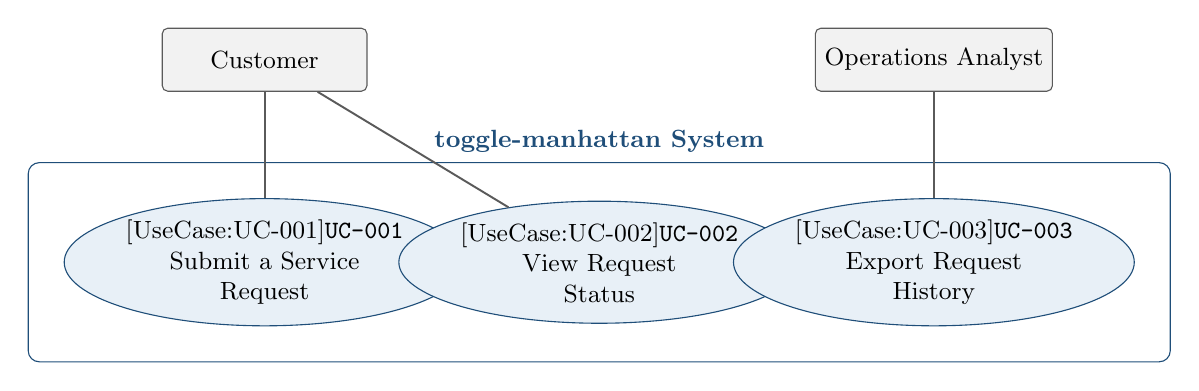
\begin{tikzpicture}[
  actor/.style={
    draw=dsnGray,
    fill=dsnGray!8,
    rounded corners=2pt,
    minimum width=2.6cm,
    minimum height=0.8cm,
    align=center,
    font=\small
  },
  use case/.style={
    ellipse,
    draw=dsnBlue,
    fill=dsnLightBlue,
    minimum width=3.8cm,
    minimum height=1.55cm,
    inner sep=1pt,
    align=center,
    font=\small
  },
  association/.style={
    draw=dsnGray,
    line width=0.7pt
  },
  system boundary/.style={
    draw=dsnBlue,
    rounded corners=4pt,
    inner sep=0.45cm
  }
]
  \node[use case] (submit) at (0,0) {\UseCaseRef{UC-001}\\Submit a Service\\Request};
  \node[use case] (status) at (4.25,0) {\UseCaseRef{UC-002}\\View Request\\Status};
  \node[use case] (export) at (8.5,0) {\UseCaseRef{UC-003}\\Export Request\\History};

  \node[system boundary, fit=(submit)(status)(export),
    label={[font=\small\bfseries, text=dsnBlue]above:\ProjectName\ System}]
    (system) {};

  \node[actor, above=1.35cm of submit] (customer) {Customer};
  \node[actor, above=1.35cm of export] (analyst) {Operations Analyst};

  \draw[association] (customer) -- (submit);
  \draw[association] (customer) -- (status);
  \draw[association] (analyst) -- (export);
\end{tikzpicture}

  \caption{High-level use-case diagram.}
  \label{Figure:HighLevelUseCase}
\end{figure}
\end{verbatim}

\section{Building the PDF}

TikZ diagrams compile directly when their source files are included by the
owning chapters. The toolchain requires:

\begin{itemize}
  \item a LaTeX distribution containing TikZ/PGF, \texttt{pdflatex},
  \texttt{bibtex}, and \texttt{latexmk};
  \item the \texttt{makeglossaries} and \texttt{makeindex} commands.
\end{itemize}

\subsection{Installing the Tools on macOS}

The full MacTeX distribution is recommended because it includes the LaTeX tools and packages used by this template. Complete these steps from an administrator account:

\begin{enumerate}
  \item Open Terminal and install Apple's command-line tools, which provide \texttt{make}:
\begin{verbatim}
xcode-select --install
\end{verbatim}
  Complete the installer dialog before continuing.

  \item Install Homebrew by following the current instructions at \url{https://brew.sh/}. Then install MacTeX, which includes TikZ:
\begin{verbatim}
brew install --cask mactex
\end{verbatim}
  MacTeX may instead be downloaded directly from \url{https://tug.org/mactex/}.

  \item Close and reopen Terminal so the MacTeX command-line tools are added to the system path.

  \item Verify that every required command is available:
\begin{verbatim}
command -v make pdflatex bibtex \
  makeglossaries makeindex latexmk
kpsewhich tikz.sty
\end{verbatim}
  Each command shall print a path. A missing line identifies the tool or TikZ
  package that still needs to be installed or added to the system path.
\end{enumerate}

\subsection{Installing the Tools on Windows}

Use a current Windows 10 or Windows 11 computer and complete these steps:

\begin{enumerate}
  \item Download and run the Basic MiKTeX Installer from \url{https://miktex.org/howto/install-miktex}. Choose a private per-user installation when appropriate and select \emph{Always install missing packages on-the-fly} for a computer with Internet access.

  \item Open MiKTeX Console, check for updates, and install them. If \texttt{latexmk} is not found during verification, use the Packages page in MiKTeX Console to install the \texttt{latexmk} package.

  \item Close and reopen PowerShell, then verify the required commands:
\begin{verbatim}
Get-Command pdflatex,bibtex
Get-Command makeglossaries,makeindex,latexmk
kpsewhich tikz.sty
\end{verbatim}
  Each tool shall produce a command record. A command-not-found error identifies a missing installation or system-path entry.
\end{enumerate}

On an organization-managed computer, authors shall ask the system administrator
before installing software or changing a managed execution policy.

\subsection{Installing the Tools on Ubuntu or Debian Linux}

Open a terminal and install TikZ/PGF, GNU Make, Latexmk, and a TeX
Live set that contains the other packages used by this template:

\begin{verbatim}
sudo apt update
sudo apt install make latexmk texlive-pictures \
  texlive-latex-extra \
  texlive-fonts-recommended texlive-bibtex-extra \
  texlive-extra-utils
\end{verbatim}

Verify the required commands:

\begin{verbatim}
command -v make pdflatex bibtex \
  makeglossaries makeindex latexmk
kpsewhich tikz.sty
\end{verbatim}

For another Linux distribution, install the equivalent TikZ/PGF, GNU
Make, Latexmk, and full or extended TeX Live packages with its package manager.

\subsection{AI-Agent Installation}
\label{Section:AIAgentInstallation}

An AI coding agent can inspect the host, identify missing commands, request
approval for system changes, install the appropriate packages, and verify the
build. Give the agent the project directory and the following reusable request:

\begin{verbatim}
In this LaTeX project, inspect the build files and determine
which operating system and package manager are available.
Verify TikZ with `kpsewhich tikz.sty`, and verify make,
pdflatex, bibtex, makeglossaries, makeindex, and latexmk.
Install only missing tools using the
platform's standard package manager. Ask for approval before
administrator-level, system-wide, or networked installation.
Do not replace project sources or remove user files. After
installation, compile included TikZ sources, run the full platform
build, inspect the log for errors, unresolved
references, and overfull boxes, and report the generated PDF.
\end{verbatim}

If the agent cannot install software, ask it to report the exact missing
command, the attempted verification, and platform-specific installation
instructions. Never give an agent an unrestricted instruction to delete build
directories or modify system security policy.

\subsection{Building on macOS and Linux}

From the template directory, run:

\begin{verbatim}
make -f makefileMacLinux pdf
\end{verbatim}

Use \texttt{make -f makefileMacLinux clean} to remove generated build files while preserving authored sources and the final PDF.

\subsection{Building with Windows PowerShell}

From PowerShell in the template directory, run:

\begin{verbatim}
.\makefilePowerShell.ps1 -Action pdf
\end{verbatim}

Use \texttt{-Action clean} in place of \texttt{-Action pdf} to remove generated build files. If local execution policy prevents scripts from running, use an approved organizational policy or allow scripts only for the current PowerShell process:

\begin{verbatim}
Set-ExecutionPolicy -Scope Process Bypass
.\makefilePowerShell.ps1 -Action pdf
\end{verbatim}

\subsection{Manual Build Sequence}

When the platform build script is unavailable, run the following commands from
the template directory. The final two LaTeX passes resolve tables of contents,
citations, glossary links, the index, and cross-references.

Included TikZ sources require no separate rendering command; \texttt{pdflatex}
compiles them with their owning chapters:

\begin{verbatim}
pdflatex -interaction=nonstopmode -halt-on-error tgmManual.tex
bibtex tgmManual
makeglossaries tgmManual
makeindex tgmManual.idx
pdflatex -interaction=nonstopmode -halt-on-error tgmManual.tex
pdflatex -interaction=nonstopmode -halt-on-error tgmManual.tex
\end{verbatim}

\subsection{Build Verification and Troubleshooting}

Confirm that the output PDF opens, all expected chapters and appendices appear,
the glossary and index are populated, hyperlinks reach their targets, and no
table or figure is clipped. Search \texttt{tgmManual.log} for fatal errors,
undefined references, missing files, and overfull boxes. Common remedies are:

\begin{itemize}
\item open a new terminal after installation so its search path is refreshed;
\item on macOS, verify that \texttt{/Library/TeX/texbin} is on the search path;
\item rerun the complete build after adding citations, glossary entries, index
entries, figures, labels, or references;
\item compile and inspect the owning chapter after changing a TikZ source;
\item install the named LaTeX package when the log reports a missing
\texttt{.sty} file.
\end{itemize}

\section{Authoring Rules}

\begin{itemize}
\item Add the newest approved change to the top of the document history.
\item Introduce specialized terms through the glossary and use them consistently.
\item Give every controlled artifact a stable explicit ID.
\item Use \texttt{shall} only for binding requirements.
\item Keep normative requirements separate from explanation and examples.
\item Apply the approved project namespace to every new project-owned file as
specified in \hyperref[Table:DocumentAuthoringRequirements]{the
document-authoring requirements}.
\item Use TikZ for all diagrams. Store every source in
\path|TikZ/<includingFileBaseName>/| and name it
\path|<nameSpace><DrawingName>.tex|.
\item Include each TikZ source from its owning chapter in a numbered figure
with a caption and stable label, and reference that figure in the chapter text.
\item Compile and inspect the PDF after structural or table changes.
\end{itemize}

\section{Citations and Bibliography}

Store controlled reference records in \texttt{tgmReferences.bib}. Cite a
source from a chapter with a stable BibTeX key:

\begin{verbatim}
\cite{ISO29148}
\end{verbatim}

The main file applies the style and prints one document-level bibliography:

\begin{verbatim}
\bibliographystyle{IEEEtran}
\bibliography{tgmReferences}
\end{verbatim}

Both platform build scripts run BibTeX automatically.

Bibliography entries support claims and definitions; they do not replace
project-owned requirements, architecture decisions, test procedures, or
approval evidence.

\section{Selective Builds}

For a large project, LaTeX's \verb|\includeonly| command may select chapters
during drafting. The main file contains a commented example:

\begin{verbatim}
% \includeonly{
%   prologue,
%   tgmRequirements,
%   tgmTests
% }
\end{verbatim}

Remove the leading comment characters and list include names without the
\texttt{.tex} extension. LaTeX can retain cross-references and citations from
omitted chapters by reading their existing auxiliary files, but those files
may be absent or stale. Selective builds are therefore drafting aids only.
Hyperref may also report missing destinations for links into deliberately
omitted chapters; these draft warnings shall disappear in the full build.
Comment out the complete \verb|\includeonly| block and run a full build before
verification or release so missing chapters, references, glossary entries,
citations, and evidence cannot be hidden.

\chapter{Embedded Systems Tailoring Profile}
\ChapterLabel{EmbeddedSystemsProfile}
\index{domain tailoring profile!embedded systems}
\index{embedded systems}
\index{hardware--software co-design}

\section{How to Use This Appendix}
This appendix tailors the generic architecture template for systems in which
software interacts directly with dedicated hardware, constrained computing
resources, physical processes, or real-time events. It applies to bare-metal
firmware, real-time operating system (RTOS) products, embedded Linux systems, programmable
logic, hardware--software products, and other cyber-physical systems.

The profile augments the core template; it does not create a second
architecture specification. Project-specific requirements, interfaces,
decisions, diagrams, tests, and evidence shall remain in their authoritative
core chapters. When this profile applies, retain this appendix as the
authoritative tailoring guide, record the applicability decision in
\ChapterRef{DevelopmentPlan}, and use the additional concerns below when
creating and reviewing the core content. Remove this appendix from an
instantiated project only when an authorized human records that the profile is
not applicable.

\section{Applicability}
\label{Section:EmbeddedProfileApplicability}
Apply this profile when one or more of the following conditions is present:

\begin{itemize}
\item software executes on a dedicated processor, microcontroller, system on
chip, field-programmable device, or purpose-built computing module;
\item behavior depends on interrupts, deadlines, deterministic scheduling,
physical signals, sensors, actuators, or control loops;
\item CPU, memory, storage, bus bandwidth, energy, or thermal resources are
materially constrained;
\item the product requires hardware bring-up, boot firmware, board support,
device drivers, manufacturing provisioning, calibration, or field firmware
updates; or
\item safety, reliability, environmental, physical-security, certification,
or component-lifecycle concerns affect the architecture.
\end{itemize}

The applicability decision shall identify the embedded platform class, the
reason the profile applies, the hardware revisions in scope, and any other
domain profiles used concurrently. A project may combine this profile with a
future safety-critical, high-security, cloud, mobile, or machine-learning
profile. Each profile remains guidance; controlled project facts stay in the
core chapters.

\section{Core-Chapter Tailoring Map}
Use Table~\ref{Table:EmbeddedTailoringMap} to place each embedded concern in
one authoritative location.

\small
\begin{tabularx}{\linewidth}{L{4.2cm}Y}
\caption{Embedded-Systems Core-Chapter Tailoring Map\label{Table:EmbeddedTailoringMap}}\\
\toprule
\textbf{Core Chapter} & \textbf{Embedded-System Additions}\\
\midrule
\endfirsthead
\multicolumn{2}{l}{\small\itshape Embedded-Systems Core-Chapter Tailoring Map (continued)}\\
\toprule
\textbf{Core Chapter} & \textbf{Embedded-System Additions}\\
\midrule
\endhead
\bottomrule
\endlastfoot
Development Plan & Record the profile decision, hardware and firmware roles,
toolchain ownership, hardware availability, prototypes, certification gates,
manufacturing dependencies, and component-lifecycle risks.\\
System Context & Define the hardware--software boundary, physical environment,
sensors, actuators, operators, service tools, external buses, power sources,
and upstream or downstream systems.\\
User Stories and Use Cases & Include installation, startup, shutdown,
calibration, diagnostics, maintenance, update, recovery, degraded operation,
manufacturing, and service interactions where applicable.\\
Requirements & Add timing, resource, power, interface, boot, recovery, safety,
security, reliability, environmental, diagnostics, update, manufacturing, and
regulatory obligations.\\
Architecture Views & Document hardware--software allocation, firmware layers,
execution contexts, states, timing, memory, deployment, data and signal flow,
power modes, faults, and recovery.\\
Implementation & Identify processor and board revisions, boot chain, BSP, HAL,
RTOS or operating system, compiler, linker, SDK, libraries, generated code,
linker scripts, build variants, image formats, and programming tools.\\
Tests, Verification, and Validation & Add target execution, static analysis,
timing analysis, SIL, PIL, HIL, fault injection, power, environmental,
hardware-revision, update, recovery, and retained-evidence activities.\\
Release & Identify released hardware revisions, firmware images, hashes,
configuration data, programming instructions, compatibility, rollback,
manufacturing release, service provisions, and known limitations.\\
\end{tabularx}
\normalsize

\section{Hardware--Software Boundary and Allocation}
The System Context and architecture chapters shall identify every processor,
memory device, programmable component, peripheral, sensor, actuator, bus,
power domain, and external physical interface that materially constrains the
software. Define which behavior is implemented in hardware, firmware,
programmable logic, operating-system services, application software, or an
external system. Record alternatives and trade-offs for significant
allocation decisions.

For each allocated function, identify its driving requirements, execution
platform, inputs, outputs, timing needs, failure behavior, update boundary,
and verification method. Do not treat a vendor module, BSP, HAL, RTOS, device
driver, or generated component as an unexamined implementation detail when it
affects required behavior.

\section{Embedded Requirement Categories}
Table~\ref{Table:EmbeddedRequirementCategories} is a checklist of common
embedded requirement categories. It does not introduce new requirement ID
families. Classify each requirement in the existing family that best describes
its primary obligation. Propose a new family only through the controlled
procedure in \ChapterRef{Requirements}. Apply the domain-profile translation
rule in Section~\ref{Section:DomainProfileRequirements}: every applicable
embedded concern shall map to a project requirement, an existing requirement,
or an approved Not Applicable decision with rationale.

\small
\begin{tabularx}{\linewidth}{L{3.7cm}Y}
\caption{Embedded-System Requirement Categories\label{Table:EmbeddedRequirementCategories}}\\
\toprule
\textbf{Category} & \textbf{Questions the Requirements Shall Resolve}\\
\midrule
\endfirsthead
\multicolumn{2}{l}{\small\itshape Embedded-System Requirement Categories (continued)}\\
\toprule
\textbf{Category} & \textbf{Questions the Requirements Shall Resolve}\\
\midrule
\endhead
\bottomrule
\endlastfoot
Functional behavior & What observable control, sensing, computation,
communication, diagnostic, maintenance, and recovery behavior is required?\\
Timing and real time & What deadlines, periods, latency, jitter, sequencing,
startup, shutdown, and worst-case response limits apply?\\
Processing resources & What CPU utilization, execution-time, core-affinity,
interrupt-latency, and scheduling limits apply?\\
Memory and storage & What flash, RAM, stack, heap, nonvolatile storage,
retention, endurance, and memory-protection limits apply?\\
Power and thermal & What operating, sleep, peak, average, battery-life,
wake-up, brownout, thermal, and power-transition behavior is required?\\
Hardware interfaces & What electrical levels, pin assignments, connectors,
buses, protocols, rates, units, ranges, scaling, resolution, endianness, and
error behavior apply?\\
Boot and initialization & What boot sources, ordering, self-tests, startup
times, configuration checks, and failure responses are required?\\
Reset and recovery & What events cause reset, retry, failover, degraded mode,
safe state, rollback, or operator intervention?\\
Safety & What hazards, safety functions, safe states, diagnostic coverage,
independence, and integrity constraints apply?\\
Security & What root of trust, secure boot, image authentication, device
identity, key provisioning, access control, debug-port, anti-rollback, and
physical-attack provisions apply?\\
Reliability and availability & What service life, duty cycle, fault tolerance,
watchdog, data-integrity, availability, maintainability, and recovery targets
apply?\\
Environmental & What temperature, humidity, vibration, shock, altitude,
electromagnetic, contamination, ingress, and storage conditions apply?\\
Diagnostics and observability & What logs, counters, health indicators, fault
codes, traces, test points, telemetry, and service interfaces are required?\\
Calibration and configuration & What values are configurable or calibrated;
who controls them; how are range, integrity, compatibility, and provenance
maintained?\\
Firmware update & What transport, authentication, atomicity, compatibility,
interruption, rollback, recovery, audit, and field-service behavior applies?\\
Manufacturing and provisioning & What programming, serialization, key
injection, calibration, end-of-line testing, traceability, and acceptance data
is required?\\
Regulatory and certification & What standards, evidence, configuration
controls, independence, analysis, and approval obligations apply?\\
Component lifecycle & What approved components, alternates, lead-time,
obsolescence, silicon errata, vendor support, and redesign constraints apply?\\
\end{tabularx}
\normalsize

Each embedded requirement shall retain the normal priority, lifecycle status,
In Version value, use-case mapping, and test-case mapping. Quantitative limits
shall state units, applicable operating conditions, tolerance, and verification
method. Avoid terms such as ``fast,'' ``low power,'' or ``robust'' without a
measurable acceptance boundary.

\section{Required Architecture Views}
Select views according to risk and complexity, and explain any omitted view
that would normally apply. Create diagrams with TikZ and store them under the
owning core chapter.

\small
\begin{tabularx}{\linewidth}{L{4.0cm}Y}
\caption{Candidate Embedded-System Architecture Views\label{Table:EmbeddedArchitectureViews}}\\
\toprule
\textbf{View} & \textbf{Content}\\
\midrule
\endfirsthead
\multicolumn{2}{l}{\small\itshape Candidate Embedded-System Architecture Views (continued)}\\
\toprule
\textbf{View} & \textbf{Content}\\
\midrule
\endhead
\bottomrule
\endlastfoot
Hardware block view & Processing, memory, programmable logic, peripherals,
clock, reset, power, sensors, actuators, and external connections.\\
Hardware--software allocation & Required functions allocated to hardware,
firmware layers, programmable logic, or external systems.\\
Firmware layering & Bootloader, BSP, HAL, drivers, RTOS or kernel, middleware,
services, application, and diagnostic boundaries.\\
Boot and update sequence & Trust chain, initialization order, self-tests,
configuration loading, update, rollback, and recovery paths.\\
Execution-context view & Cores, processes, tasks, threads, interrupt service
routines, priorities, scheduling, synchronization, and shared resources.\\
State and mode view & Operational, maintenance, calibration, degraded, safe,
sleep, update, and fault states with permitted transitions.\\
Timing view & Periods, deadlines, latency, jitter, sequencing, bus transactions,
control-loop timing, and worst-case paths.\\
Memory view & Address spaces, partitions, executable regions, stacks, heaps,
DMA buffers, retained data, memory protection, and nonvolatile layout.\\
Data and signal flow & Units, scaling, sample rates, filtering, validity,
ownership, persistence, and error propagation.\\
Deployment view & Firmware images and configuration deployed to processors,
cores, boards, hardware revisions, and manufacturing or field tools.\\
Power and thermal view & Power domains, modes, transitions, wake sources,
consumers, thermal limits, throttling, and shutdown behavior.\\
Fault-containment view & Fault-detection boundaries, watchdogs, redundancy,
degraded operation, safe states, containment, and recovery.\\
\end{tabularx}
\normalsize

\section{Interfaces and Protocols}
For every hardware or communication interface, document the physical and
logical contract together. Include connector and pin identity, direction,
electrical characteristics, protocol and version, topology, addressing,
message or register definition, data type, units, range, resolution, scaling,
endianness, update rate, timing, initialization, ownership, concurrency,
timeouts, integrity checks, invalid values, error handling, compatibility, and
verification method where applicable.

An interface table or referenced interface-control document shall have a
controlled identifier and version. Each interface requirement and test shall
link to that authority. Do not infer an electrical limit, register behavior,
reserved bit, or protocol tolerance without controlled evidence.

\section{Resource Budgets}
Maintain resource budgets whenever architecture feasibility depends on a
finite embedded resource. Table~\ref{Table:EmbeddedResourceBudget} is a generic
pattern; create one row for each controlled allocation and reconcile component
allocations with the system total.

\small
\begin{tabularx}{\linewidth}{L{2.2cm}L{2.5cm}L{2.2cm}L{2.3cm}Y}
\caption{Generic Embedded Resource Budget\label{Table:EmbeddedResourceBudget}}\\
\toprule
\textbf{Resource} & \textbf{Owner} & \textbf{Allocation} & \textbf{Measured or Estimated} & \textbf{Requirement / Evidence}\\
\midrule
\endfirsthead
\multicolumn{5}{l}{\small\itshape Generic Embedded Resource Budget (continued)}\\
\toprule
\textbf{Resource} & \textbf{Owner} & \textbf{Allocation} & \textbf{Measured or Estimated} & \textbf{Requirement / Evidence}\\
\midrule
\endhead
\bottomrule
\endlastfoot
CPU time & [task or component] & [limit and units] & [value, method, conditions] & [requirement and test IDs]\\
Flash & [image or component] & [bytes or percent] & [map-file value] & [requirement and evidence]\\
RAM & [task or component] & [bytes or percent] & [static and peak value] & [requirement and evidence]\\
Stack & [task or context] & [bytes] & [worst observed or analyzed] & [requirement and evidence]\\
Bus bandwidth & [interface or flow] & [rate and utilization] & [value and conditions] & [requirement and test IDs]\\
Power or energy & [mode or component] & [power, current, or energy] & [value and conditions] & [requirement and test IDs]\\
Thermal margin & [component or mode] & [temperature or margin] & [value and conditions] & [requirement and evidence]\\
\end{tabularx}
\normalsize

Every budget shall state the measurement or estimation conditions, margin
policy, uncertainty, owner, update trigger, and response to an exceeded
allocation. Budget evidence shall distinguish analysis, simulation,
measurement, and worst-case guarantee.

\section{Safety, Reliability, and Fault Management}
Identify hazards, failure modes, fault sources, detection mechanisms,
containment boundaries, watchdogs, redundancy, degraded modes, safe states,
recovery behavior, diagnostic coverage, and residual risk where applicable.
Trace every credited mechanism to requirements and verification evidence.

Do not claim a safety integrity level, diagnostic coverage, failure rate,
independence, or risk acceptance without the applicable analysis and
authorized approval. When a dedicated safety profile or regulated process
applies, use it together with this embedded profile and record precedence for
any conflicting rule.

\section{Embedded Security}
Define the trust boundary and lifecycle from manufacturing through
decommissioning. Address device identity, root of trust, secure boot, image
authentication, signing and key custody, provisioning, credential storage,
debug and test access, privileged interfaces, update authorization,
anti-rollback, protected configuration, security logging, recovery, physical
attack assumptions, vulnerability response, and secure decommissioning as
applicable.

Security controls shall be mapped to threats, requirements, tests, retained
evidence, and operational responsibilities. Secrets and production keys shall
not be placed in this architecture document, source repository, AI prompt, or
test artifact.

\section{Toolchain and Configuration Control}
Record the controlled hardware revisions, processor variants, compiler and
linker versions, optimization and warning settings, linker scripts, BSP, HAL,
RTOS or operating-system version, SDK, libraries, code generators, programming
tools, static-analysis tools, build variants, configuration sources, and image
formats. Identify which outputs are generated, how they are reproduced, and
which tool qualifications or validations apply.

A released firmware image shall be traceable to source revision, configuration,
toolchain, dependencies, hardware compatibility, build procedure, image hash,
and approval evidence. Changes to silicon revision, board revision, compiler,
optimization, RTOS, BSP, HAL, linker script, or generated-code input shall
trigger an impact assessment.

\section{Embedded Verification and Validation}
Select test environments according to the requirement and the confidence
needed. The verification plan may include review, static analysis, host unit
tests, software-in-the-loop (SIL), processor-in-the-loop (PIL), target tests,
hardware-in-the-loop (HIL), fault injection, timing and worst-case execution
analysis, stress, endurance, power, thermal, environmental, electromagnetic,
hardware-revision compatibility, boot, update, rollback, and recovery testing.

Each result shall identify the hardware revision, firmware version, build
configuration, tool and fixture versions, calibration state, environmental
conditions, input data, procedure, expected result, actual result, retained
evidence, and reviewer. Simulation or host-test evidence shall not be
represented as target evidence. Validation shall use representative intended
operation and stakeholders or authorized representatives.

\section{AI Tailoring Instructions}
\index{AI agent!embedded systems tailoring}
When this profile is Applicable or TBD, an AI agent shall read this appendix
with the task-specific core chapters. Before editing, it shall ask for or
confirm:

\begin{itemize}
\item the platform class: bare metal, RTOS, embedded Linux, programmable logic,
or mixed;
\item processor, board, programmable-device, and hardware revisions in scope;
\item boot chain, operating system or RTOS, BSP, HAL, SDK, compiler, linker,
and relevant third-party components;
\item external interfaces, sensors, actuators, physical environment, timing,
resource, power, safety, security, regulatory, manufacturing, update, and
service constraints; and
\item available schematics, datasheets, interface-control documents, hazard
analysis, threat analysis, test evidence, and authorized approvals.
\end{itemize}

The agent shall add embedded concerns to the initialization gap list and place
project facts only in their authoritative core chapters. It shall not invent
pinouts, register behavior, electrical limits, memory sizes, execution times,
power measurements, hardware compatibility, safety classifications, security
claims, certification evidence, or test results. It shall report missing
controlled hardware evidence and every decision requiring authorized human
approval.

Use the following request for an embedded project:

\begin{verbatim}
Read tgmAIAgentGuide.tex and tgmEmbeddedSystemsProfile.tex. Apply the
Embedded Systems Tailoring Profile to [Project Name]. Ask me to
confirm the project namespace, profile applicability, platform class,
hardware revisions, toolchain, interfaces, constraints, applicable
standards, and available evidence. Add embedded concerns to the gap
list before editing. After human review, place project-specific
requirements, architecture, diagrams, tests, and evidence only in
their authoritative core chapters. Do not invent hardware facts or
verification results. Build the complete document, inspect the log,
and visually inspect the affected PDF pages.
\end{verbatim}

\section{Embedded-Profile Completion Checklist}
Before completing embedded tailoring, confirm that:

\begin{itemize}
\item profile applicability and rationale are recorded;
\item the hardware--software boundary and function allocation are explicit;
\item timing, resources, power, interfaces, boot, recovery, safety, security,
environmental, update, manufacturing, and lifecycle concerns were assessed;
\item required embedded views and resource budgets exist or have documented
omission rationales;
\item hardware revisions, firmware versions, toolchain, build variants, and
released images are configuration controlled;
\item requirements, use cases, tests, traceability, verification, validation,
and release records have reciprocal links; and
\item the build succeeds and affected tables, diagrams, links, and page breaks
have been visually inspected.
\end{itemize}

\chapter{AI Agent Usage Guide}
\ChapterLabel{AIAgentGuide}
\index{AI agent}
\index{AI agent!context routing}
\index{AI agent!example prompts}
\index{AI agent!human review}
\index{AI agent!TikZ requirement}
\index{Appendix!AI Agent Usage Guide}

\section{How to Use This Appendix}
This appendix is the entry point for an AI agent that creates, reviews, or
maintains this architecture specification. The agent shall read this file
first, identify the requested task in
\hyperref[Table:AITaskRouting]{the task-routing table}, and load only the
authoritative sources listed for that task. It shall expand the context when a
referenced dependency, cross-cutting decision, or inconsistency requires it.

This appendix replaces substantive AI-oriented Markdown instructions. A thin
repository bootstrap may point an AI tool to this appendix, but its routing
tables, context packs, workflows, prompts, and checklists are maintained only
as LaTeX so they remain visible in the architecture book and versioned with the
specification.

\section{Governing Principles}
\index{source of truth}
The authored LaTeX files and editable diagram sources are the source of truth.
TikZ is the required source format for diagrams.
The generated PDF is a review artifact and shall not be edited directly. The
agent shall preserve one authoritative location for each fact and use links
instead of duplicating content across chapters.

An AI agent is a drafting, analysis, consistency-checking, and build assistant.
It shall use supplied project evidence, identify missing information, expose
material assumptions, and distinguish proposals from approved decisions. It
shall not invent requirements approval, implementation status, test results,
verification evidence, validation evidence, waivers, or release authorization.

\section{AI Quick Start}
\label{Section:AIQuickStart}
\index{AI agent!quick start}

\begin{enumerate}
\item Read this appendix and identify the requested outcome.
\item Before creating or renaming a project-owned file, ask for or confirm the
project file namespace. Do not invent it; use the confirmed namespace for every
file created during the task.
\item Inspect \hyperref[Table:DomainProfileApplicability]{the domain-profile
applicability table} and \hyperref[Table:ProjectDomainProfiles]{the project
profile decisions}. Ask an authorized human to resolve any unreviewed profile
selection. Load every Applicable or TBD profile affected by the task.
\item Select the closest entry in
\hyperref[Table:AITaskRouting]{the task-routing table}.
\item Read the listed primary files and the applicable context pack. Read
\texttt{tgmManual.tex} when document metadata, macros, inclusion order, or
build structure is affected.
\item Inspect available project evidence and report conflicts, missing facts,
and consequential assumptions. Ask for a human decision when an answer would
materially change scope, architecture, safety, security, cost, schedule, or
release readiness.
\item Make narrowly scoped changes in the authoritative files. Preserve stable
IDs and update every affected reciprocal mapping.
\item Add a linked document-history entry for an approved document change and
record material AI interactions in \ChapterRef{AIPromptLog}.
\item Run the complete build, inspect the log, render affected PDF pages, and
complete \hyperref[Table:AICompletionChecklist]{the completion checklist}.
\end{enumerate}

\section{Repository AI Bootstrap}
\label{Section:AIRepositoryBootstrap}
\index{AI agent!repository bootstrap}
\index{AGENTS.md}
\index{CLAUDE.md}
\index{SKILL.md}

The LaTeX architecture is authoritative, but an AI tool may require a
repository-level discovery file before it knows where to find these
instructions. Create a thin bootstrap file for each AI tool that the project
actually uses. The bootstrap shall point to this chapter and the relevant
LaTeX sources; it shall not reproduce their requirements, workflows, or
architectural decisions. When policy changes, update the authoritative LaTeX
source rather than copying the change into each bootstrap file.

Tool-mandated discovery names are documented exceptions to the project file
namespace requirement. This exception applies only to the exact filename or
location required for discovery. It does not exempt files created while
performing the instructed work from the namespace requirements in
\hyperref[Table:DocumentAuthoringRequirements]{the document-authoring
requirements}.

Create only the applicable files:

\footnotesize
\begin{tabularx}{\linewidth}{L{4.5cm}Y}
\caption{Repository AI Bootstrap Files\label{Table:AIRepositoryBootstrapFiles}}\\
\toprule
\textbf{File} & \textbf{When to Create It}\\
\midrule
\endfirsthead
\multicolumn{2}{l}{\small\itshape Repository AI Bootstrap Files (continued)}\\
\toprule
\textbf{File} & \textbf{When to Create It}\\
\midrule
\endhead
\bottomrule
\endlastfoot
\texttt{AGENTS.md} & The repository is maintained with Codex or another agent
that discovers this filename.\\
\texttt{CLAUDE.md} & The repository is maintained with Claude Code.\\
\texttt{.github/copilot-}\newline\texttt{instructions.md} & The repository uses repository-wide
GitHub Copilot instructions.\\
\texttt{SKILL.md} & The repository is intentionally packaged as, or contains,
a reusable AI skill. Do not create this file merely as a second copy of
\texttt{AGENTS.md}.\\
\end{tabularx}
\normalsize

Each bootstrap file shall identify the root architecture source, point to this
chapter, require task-appropriate context loading through
\hyperref[Table:AITaskRouting]{the task-routing table}, direct architecture
policy changes back to LaTeX, and point to \ChapterRef{DocumentGuide} for
building and verification. It shall also state the confirmed project file
namespace or direct the agent to obtain it before creating project-owned files.
Use the following content as a minimal tool-neutral pattern, adapting only the
discovery-specific wrapper:

\begin{verbatim}
# AI Instructions

The authoritative software architecture is maintained in
tgmManual.tex. Before architecture-related work, read
tgmAIAgentGuide.tex and use its task-routing table to identify the
additional LaTeX chapters required for the task.

Treat the authored LaTeX and editable diagram sources as the source
of truth. Do not duplicate their requirements, conventions,
workflows, or architectural decisions in this file. When policy
changes, update the authoritative LaTeX source.

Before creating project-owned files, obtain or confirm the project
namespace required by tgmDocumentGuide.tex. Follow that guide's
build and verification instructions before completing the task.
\end{verbatim}

\section{Task Routing}
\index{AI agent!task routing}
The file lists below are minimum starting contexts, not permission to ignore a
dependency discovered during the task. A task that changes an artifact shall
also inspect every register that contains a reciprocal mapping to that
artifact.

\small
\begin{tabularx}{\linewidth}{L{4.0cm}Y}
\caption{AI Task-Routing Table\label{Table:AITaskRouting}}\\
\toprule
\textbf{Task} & \textbf{Minimum Authoritative Sources}\\
\midrule
\endfirsthead
\multicolumn{2}{l}{\small\itshape AI Task-Routing Table (continued)}\\
\toprule
\textbf{Task} & \textbf{Minimum Authoritative Sources}\\
\midrule
\endhead
\midrule
\multicolumn{2}{r}{\small\itshape Continued on next page}\\
\endfoot
\bottomrule
\endlastfoot
Initialize a project & \texttt{tgmManual.tex}, \texttt{prologue.tex}, \texttt{tgmIntroduction.tex}, \texttt{tgmDevelopmentPlan.tex}, \texttt{tgmSystemContext.tex}, each proposed or selected domain profile, and the supplied project evidence.\\
Tailor an embedded system & \texttt{tgmEmbeddedSystemsProfile.tex},
\texttt{tgmDevelopmentPlan.tex}, \texttt{tgmSystemContext.tex},
\texttt{tgmRequirements.tex}, the affected architecture and interface
chapters, \texttt{tgmTests.tex}, \texttt{tgmTraceability.tex}, and the
controlled hardware and project evidence.\\
Create repository AI bootstrap files & \texttt{tgmAIAgentGuide.tex},
\texttt{tgmDocumentGuide.tex}, \texttt{tgmManual.tex}, evidence identifying the
AI tools used by the project, and each tool's required discovery filename.\\
Develop user stories & \texttt{tgmSystemContext.tex}, \texttt{tgmUserStories.tex}, \texttt{tgmRequirements.tex}, and stakeholder evidence.\\
Add or change requirements & \texttt{tgmUserStories.tex}, \texttt{tgmRequirements.tex}, every Applicable or TBD domain profile, \texttt{tgmUseCases.tex}, \texttt{tgmTests.tex}, \texttt{tgmTraceability.tex}, \texttt{tgmVerification.tex}, and \texttt{tgmGlossary.tex}.\\
Add or change use cases & \texttt{tgmUserStories.tex}, \texttt{tgmRequirements.tex}, \texttt{tgmUseCases.tex}, \texttt{tgmTests.tex}, and \texttt{tgmTraceability.tex}.\\
Develop or change architecture & \texttt{tgmSystemContext.tex}, \texttt{tgmRequirements.tex}, \texttt{tgmArchitectureOverview.tex}, the affected interface, logical, process, development, physical, or implementation chapters, and their \texttt{TikZ/} diagram sources.\\
Add or change tests & \texttt{tgmRequirements.tex}, \texttt{tgmUseCases.tex}, \texttt{tgmTests.tex}, \texttt{tgmTraceability.tex}, \texttt{tgmVerification.tex}, and \texttt{tgmTestEvidence.tex}.\\
Perform verification & \texttt{tgmRequirements.tex}, \texttt{tgmTests.tex}, \texttt{tgmTraceability.tex}, \texttt{tgmVerification.tex}, and controlled test evidence.\\
Perform validation & \texttt{tgmUserStories.tex}, \texttt{tgmUseCases.tex}, \texttt{tgmValidation.tex}, and controlled stakeholder evidence.\\
Prepare a release & \texttt{tgmRequirements.tex}, \texttt{tgmTraceability.tex}, \texttt{tgmVerification.tex}, \texttt{tgmValidation.tex}, \texttt{tgmRelease.tex}, and controlled release evidence.\\
Review consistency & All registers containing the affected artifact types, \texttt{tgmGlossary.tex}, \texttt{tgmDocumentHistory.tex}, and \texttt{tgmManual.tex}.\\
Compile or troubleshoot & \texttt{tgmManual.tex}, \texttt{tgmDocumentGuide.tex}, the affected chapter, its diagram sources, and the build log.\\
\end{tabularx}
\normalsize

\section{Task-Specific Context Packs}
\index{AI agent!context pack}
A context pack is a reading boundary within this appendix, not a separate file.
Use the applicable pack together with the task-routing entry.

\subsection{Domain-Profile Context}
Determine the Applicable, Not Applicable, or TBD status of every available
domain profile during initialization. An authorized human shall approve the
selection and rationale. For later tasks, load every Applicable or TBD profile
whose concerns intersect the requested change. A profile adds review concerns
and artifact expectations; project-specific facts remain in their authoritative
core chapters. When the Embedded Systems profile applies, follow
\ChapterRef{EmbeddedSystemsProfile} and add hardware, firmware, timing,
resource, power, physical-interface, safety, security, manufacturing, update,
and field-service concerns to the task context. For requirements work, apply
the controlled translation rule in
Section~\ref{Section:DomainProfileRequirements}: each applicable profile
concern shall map to a requirement, an existing requirement, or an approved
Not Applicable decision with rationale.

\subsection{Requirements Context}
Establish the system boundary and stakeholder need before proposing a
requirement. Keep each requirement singular, feasible, unambiguous, and
verifiable. Apply the identifier grammar and family definitions in
Section~\ref{Section:RequirementIdentifierConvention}. Classify its primary
family or subtype, write binding behavior with
\textbf{shall}, assign one \gls{must}, \gls{should}, \gls{could}, or
\gls{would} priority, assign one lifecycle status, and map it to at least one
use case and one test case. A requirement may be marked Done only when its
mapped tests pass, verification is complete, traceability is current, and a
controlled implementation version is known. Evaluate every Applicable or TBD
domain profile that intersects the proposed change and follow
Section~\ref{Section:DomainProfileRequirements} before completing the
requirements work.

\subsection{Use-Case Context}
Start from an actor goal and a system boundary. Give each use case its own
table, identify participating actors, preconditions, trigger, success outcome,
main flow, alternate and exception flows, postconditions, mapped requirements,
and mapped tests. Describe externally observable interaction rather than
internal implementation detail. Maintain reciprocal mappings to every related
requirement.

\subsection{Architecture Context}
Trace each architectural decision to requirements, quality attributes,
constraints, risks, and interfaces. Identify alternatives and explain the
trade-off that selected the proposed structure. Keep the context, logical,
process, development, physical, interface, and implementation views consistent.
Use TikZ for diagrams.
Store each TikZ source under its owning chapter as required by
Section~\ref{Section:TikZAuthoring}, include it from that chapter, and compile
the PDF.

\subsection{Testing and Evidence Context}
Derive tests from requirements and use cases. Define preconditions, inputs,
procedure, expected result, and retained evidence. A test definition is not a
test result. Verification records objective compliance with requirements;
validation records whether stakeholder needs are satisfied in intended use.
Never create passing evidence or approval from an expected result.

\subsection{Release Context}
Review open, in-progress, done, and retired requirements; unresolved defects;
verification and validation results; operational readiness; migration and
rollback provisions; known limitations; and required approvals. Report a gap
instead of treating missing evidence as acceptance. Only an authorized human
may approve release.

\subsection{Document-Authoring Context}
Follow \ChapterRef{DocumentGuide} for file naming, LaTeX conventions, diagrams,
installation, and builds. Update the glossary and index when introducing a
controlled term. Update document history with a link to the changed location.
Before creating or renaming a project-owned file, ask for or confirm the
project file namespace and apply it consistently in accordance with
\hyperref[Table:DocumentAuthoringRequirements]{the document-authoring
requirements}.
Every TikZ source shall satisfy the path, inclusion, caption, label, and
reference requirements in Section~\ref{Section:TikZAuthoring}. Do not edit
generated auxiliary files or the PDF directly.

\section{Mandatory Consistency Rules}
\index{AI agent!consistency rules}

\begin{enumerate}
\item Preserve every stable ID. Do not reuse an ID belonging to a retired or
deleted proposal.
\item Use the scope and family codes in
Section~\ref{Section:RequirementIdentifierConvention}. Before using an
undefined scope or family, propose its code, name, boundary, rationale, and
examples; check for semantic overlap and identifier collision; obtain
authorized-human approval; and update the convention, category catalog, this
guide, and the applicable register. Do not rename existing IDs when extending
the convention.
\item Use \textbf{shall} for binding requirements. Use priority terms only in
the Priority field and with the definitions in the glossary.
\item Give every requirement a priority, status, In Version value, use-case
mapping, and test-case mapping.
\item Enter \NoVersion\ when a requirement is not Done and no completed
implementation version applies.
\item Maintain reciprocal mappings among user stories, requirements, use
cases, tests, traceability, verification, and validation.
\item Do not copy one controlled statement into several authoritative
locations. Link to its stable ID.
\item Retain retired requirements and their history. Record the rationale and
replacement when applicable.
\item Use project evidence for factual claims. Label an unsupported suggestion
as a proposal and report the evidence needed to decide it.
\item Record each domain profile as Applicable, Not Applicable, or TBD with an
authorized decision and rationale. Load every Applicable or relevant TBD
profile; do not duplicate project facts in the profile appendix.
\item Before creating or renaming any project-owned file, ask for or confirm
the project \texttt{\textless nameSpace\textgreater}; do not invent it. Prefix
every new project-owned file name with the confirmed namespace.
\item Use TikZ for every diagram. Every TikZ source shall use the directory
\begin{center}
\texttt{TikZ/\textless includingFileBaseName\textgreater/}
\end{center}
and shall be named \path|<nameSpace><DrawingName>.tex|. The directory shall exactly match the base
name of the LaTeX file containing its \verb|\input| command. The including
chapter shall place it in a
numbered figure, add a descriptive caption and stable label, and reference the
figure in its text.
\item Link every document-history entry to the location where the change
occurred.
\item Compile after structural, cross-reference, glossary, index, diagram, or
table changes and visually inspect the affected pages.
\end{enumerate}

\section{Standard AI Workflows}
\label{Section:AIArchitectureWorkflow}
\index{AI agent!architecture workflow}

\subsection{Initialize a Project}
Ask an authorized human for the project file namespace, or confirm an already
configured namespace, before creating or renaming files. Do not invent it.
Replace \verb|\FileNamespace|, project metadata, and bracketed placeholders
only from supplied facts, then apply the namespace to every new project-owned
file.
Identify available domain profiles and ask an authorized human to confirm each
profile's applicability. Record the decisions in
\hyperref[Table:ProjectDomainProfiles]{the project profile table}. Include each
Applicable or TBD profile in the initialization context; remove an
inapplicable profile appendix only after its decision is recorded.
Create a gap list covering purpose, scope, stakeholders, system boundary,
interfaces, constraints, quality attributes, risks, evidence, and approvals.
Resolve consequential gaps before developing detailed artifacts. Work in
dependency order from context and needs through requirements, use cases,
architecture, tests, evidence, and release.

\subsection{Add or Change a Requirement}
Identify the originating need and affected use cases. Draft a singular
verifiable obligation, select its scope, primary family, priority, and status,
and assign a stable ID using
Section~\ref{Section:RequirementIdentifierConvention}. If no defined scope or
family fits, complete the proposal and human-approval procedure before
assigning the ID. Add or update mapped use cases and tests, then update
traceability and verification. Confirm every link in both directions and add a
linked history entry.

\subsection{Add or Change a Use Case}
Identify the actor goal, system boundary, and mapped requirements. Complete one
use-case table with success, alternate, and exception behavior. Add mapped
tests, update requirement mappings and traceability, and confirm that no flow
introduces an unrecorded requirement.

\subsection{Develop or Change Architecture}
Identify the requirements and quality attributes that drive the decision.
Describe alternatives, trade-offs, risks, interfaces, and the selected
structure. Update every affected architectural view and diagram. Confirm that
the proposed design neither omits a driving requirement nor silently adds an
unapproved constraint.

\subsection{Add Tests or Evidence}
Derive each test from mapped requirements and use-case flows. Define repeatable
steps and objective expected results. Link retained evidence only after an
actual execution. Update verification or validation records without converting
an expected outcome into a claimed result.

\subsection{Review and Prepare a Release}
Audit IDs, mappings, statuses, versions, unresolved assumptions, verification,
validation, operational readiness, and release criteria. Report contradictions
and missing evidence. Prepare a release recommendation for human approval; do
not approve the release.

\section{Example AI Requests and Prompts}
\label{Section:AIExamplePrompts}
\index{AI agent!example prompts}
Replace bracketed text with project facts. A prompt does not override this
guide, the controlled project evidence, or human approval boundaries.

\subsection{Initialize the Architecture Book}
\begin{verbatim}
Read tgmAIAgentGuide.tex and use the Initialize a Project workflow
for [Project Name]. Review the supplied project evidence and create
a gap list before editing. Identify missing scope, stakeholders,
interfaces, constraints, quality attributes, risks, evidence, and
approvals. Identify the available domain profiles and ask me to
confirm whether each is Applicable, Not Applicable, or TBD. Read each
Applicable or relevant TBD profile and add its concerns to the gap
list. After the gap list is reviewed, replace only supported
placeholders and develop the document in dependency order. Compile
the complete PDF and report unresolved human decisions.
\end{verbatim}

\subsection{Tailor an Embedded System}
\begin{verbatim}
Read tgmAIAgentGuide.tex and tgmEmbeddedSystemsProfile.tex. Apply the
Embedded Systems Tailoring Profile to [Project Name]. Ask me to
confirm the project namespace, profile applicability, platform class,
hardware revisions, toolchain, interfaces, constraints, applicable
standards, and available evidence. Add embedded concerns to the gap
list before editing. After human review, place project-specific
requirements, architecture, diagrams, tests, and evidence only in
their authoritative core chapters. Do not invent hardware facts or
verification results. Build the complete document, inspect the log,
and visually inspect the affected PDF pages.
\end{verbatim}

\subsection{Create Repository AI Bootstrap Files}
\begin{verbatim}
Read the Repository AI Bootstrap section in tgmAIAgentGuide.tex and
treat that LaTeX chapter as authoritative. Confirm which AI tools
this repository uses and the project file namespace. Create only the
applicable repository discovery files, such as AGENTS.md or
CLAUDE.md. Create SKILL.md only when the repository is intentionally
packaged as, or contains, a reusable skill. Keep every bootstrap file
short: point to tgmManual.tex, tgmAIAgentGuide.tex, the task-routing
table, and tgmDocumentGuide.tex. Do not duplicate architecture rules.
Verify that each file directs architecture-related changes back to
the authoritative LaTeX sources.
\end{verbatim}

\subsection{Develop Requirements}
\begin{verbatim}
Read tgmAIAgentGuide.tex and follow the Requirements context and
workflow. Load every Applicable or TBD domain profile that intersects
the work. From the approved objectives and user stories, propose
singular, feasible, and verifiable requirements. Classify each one,
use shall for the binding obligation, assign one priority and one
status, and map it to at least one use case and test case. Do not
complete requirements work until each applicable profile concern maps
to a new or existing requirement, or to an approved Not Applicable
decision with rationale. Do not mark work Done or assign an
implementation version without evidence.
Update reciprocal mappings, history, and the index; then build and
inspect the affected pages.
\end{verbatim}

\subsection{Develop Use Cases}
\begin{verbatim}
Read tgmAIAgentGuide.tex and follow the Use-Case context and
workflow. Derive use cases from the approved actor goals and mapped
requirements. Give each use case its own table with actors, trigger,
preconditions, main flow, alternate and exception flows, outcome,
postconditions, requirements, and tests. Maintain reciprocal links
and report any flow that requires a new requirement. Build and
inspect the affected pages.
\end{verbatim}

\newpage
\subsection{Develop an Architecture Decision}
\thispagestyle{fancy}
\begin{verbatim}
Read tgmAIAgentGuide.tex and follow the Architecture context and
workflow for [decision or subsystem]. Identify driving requirements,
quality attributes, constraints, interfaces, and risks. Compare
reasonable alternatives and document the trade-off supporting the
proposed choice. Update every affected architecture view and editable
diagram source. Do not present the proposal as approved. Compile the
document and inspect all affected diagrams and pages.
\end{verbatim}

\subsection{Develop Tests and Traceability}
\begin{verbatim}
Read tgmAIAgentGuide.tex and follow the Testing and Evidence context.
For [requirements or use cases], define repeatable tests with inputs,
preconditions, steps, expected results, and required evidence. Update
all reciprocal mappings and the traceability matrix. Do not invent an
execution result or mark verification complete. Compile the document,
check references, and inspect the affected tables.
\end{verbatim}

\subsection{Review Release Readiness}
\begin{verbatim}
Read tgmAIAgentGuide.tex and follow the Release context and workflow
for [release]. Audit requirement status and implementation versions,
traceability, verification, validation, defects, operations, rollback,
known limitations, and approvals. Separate confirmed evidence from
gaps and assumptions. Prepare a release-readiness recommendation for
human review, but do not approve release. Build and inspect the final
document.
\end{verbatim}

\section{Human Decisions and Information Boundaries}
\index{AI agent!human review}
An authorized human shall approve scope, requirements, architecture decisions,
security and privacy posture, safety decisions, evidence sufficiency, waivers,
validation conclusions, and release. The agent shall present alternatives and
evidence without claiming that review has occurred.

Do not provide an AI agent with credentials, secrets, personal data,
production data, export-controlled material, or other information it is not
authorized to process. Before using external sources, confirm that the task
permits network access and that the source may be incorporated. Record material
prompts, assumptions, corrections, and unresolved issues in
\ChapterRef{AIPromptLog}.

\section{Completion Checklist}
\index{AI agent!completion checklist}
\small
\begin{tabularx}{\linewidth}{L{3.5cm}Y}
\caption{AI-Assisted Change Completion Checklist\label{Table:AICompletionChecklist}}\\
\toprule
\textbf{Area} & \textbf{Required Completion Evidence}\\
\midrule
\endfirsthead
\multicolumn{2}{l}{\small\itshape AI-Assisted Change Completion Checklist (continued)}\\
\toprule
\textbf{Area} & \textbf{Required Completion Evidence}\\
\midrule
\endhead
\bottomrule
\endlastfoot
Scope & The requested outcome is complete; unrelated chapters and user changes remain untouched.\\
Domain profiles & Every available profile has an authorized applicability
decision and rationale; every Applicable or relevant TBD profile was included
in the task context, and project facts remain in core chapters.\\
Evidence & New factual statements are supported by supplied or controlled evidence; proposals, assumptions, and unknowns are identified.\\
Language & Binding requirements use shall; priority and status use the controlled terms and definitions.\\
Identifiers & Stable IDs follow the documented scope and family convention, remain unique, and are neither renumbered nor reused; every new scope or family has its definition and authorized-human approval recorded before use.\\
File names & The project namespace was supplied or explicitly confirmed; every newly created project-owned file begins with it, and no namespace was invented.\\
AI bootstrap & Every applicable repository AI discovery file is a thin pointer
to the authoritative LaTeX architecture; tool-mandated filenames are documented
exceptions, and no architecture rules are duplicated in Markdown.\\
Traceability & Every changed requirement, use case, test, verification record, and validation record has complete reciprocal mappings.\\
History & The newest approved document change appears at the top of document history and links to the changed location.\\
Glossary and index & New controlled terms and important concepts are defined and indexed where applicable.\\
Diagram source & Every diagram uses TikZ; each TikZ directory exactly matches its including LaTeX file's base name, each drawing file begins with the project namespace, and the drawing is included, captioned, labeled, and referenced.\\
Build & The complete platform build succeeds; citations, glossary, index, diagrams, and cross-references are regenerated.\\
Log review & No fatal error, undefined reference, duplicate label, missing file, or unresolved layout warning remains.\\
Visual review & Affected PDF pages show readable tables, correct page breaks, current diagrams, working headings, and no clipped or overlapping content.\\
Human review & Decisions requiring authority are clearly identified and are not represented as approved without evidence.\\
\end{tabularx}
\normalsize

\chapter{AI Prompt Log}
\ChapterLabel{AIPromptLog}
\section{How to Use This Appendix}
Use this log when AI assistance materially affects requirements, architecture, code, tests, or release evidence. Record enough context for a reviewer to understand the input, output, assumptions, and human corrections.
\section{Example Record}
Date: \textit{[timestamp]}; Tool and model: \textit{[name]}; Input: \textit{[requirements and constraints supplied]}; Task: \textit{[requested output]}; Human review and corrections: \textit{[summary]}; Unresolved assumptions: \textit{[list or none]}.

\section{Requirement Scope or Family Extension Record}
When an AI-assisted change proposes a requirement scope or family that is not
already defined, record the proposed uppercase code, full name, decision
boundary, rationale, representative examples, semantic-overlap review,
identifier-collision check, affected register and category-catalog changes, and
the authorized human's approval or rejection. Do not assign an identifier from
the proposed scope or family before approval.

\section{Project Initialization Record}
\label{Section:PromptLogInitialization}
Date: October 14, 2026; Tool and model: Anthropic Claude Code (Claude Opus
5.5); Input: the template initialization request in
Section~\ref{Section:InitializeNewProject}, the project name
\ProjectName, file namespace \texttt{tgm}, AI tool selection (Claude Code
only; no reusable skill), Embedded Systems profile marked Applicable, document
metadata, and the statement that the system controls the opening and closing
of a curtain through an undecided method (physical controller or phone
application); Task: produce an initialization gap list, then initialize the
project copy, create applicable AI bootstrap files, and build and inspect the
document; Human review and corrections: the requester confirmed the namespace,
AI tools, profile applicability, and metadata, and stated that no further
project evidence exists; Unresolved assumptions: none adopted. Open decisions
are listed in \hyperref[Section:OpenContextItems]{the open context items}; the
authorized approver and the embedded-profile decision owner were initially
TBD. Follow-up decisions on October 14, 2026: Stel Angelidis is the authorized
approver and approved the Embedded Systems profile decision; the control
method is both a physical controller and a phone application; the embedded
platform class remains TBD; Claude Code history entries use the initials
CLAUDE; the stakeholders are people who want a low-cost, non-privacy-invading
IoT curtain closer; privacy means no data collection about individual people
and no cameras or microphones; components cost no more than USD 20 (cost basis
TBD); the system runs on a microcontroller, with all other platform details
TBD. The
template's example requirements, use cases, tests, and registers remain
unchanged as generic examples and are not project content.

\chapter{Test Evidence}
\ChapterLabel{TestEvidence}
\section{How to Use This Appendix}
Store or reference detailed test and verification evidence here when it would make the main chapters difficult to read. Evidence must identify the artifact, result, environment, date, and product revision.
\section{Example Evidence Record}
Test: \textit{TC-001}; Result: \textit{Pass}; Environment: \textit{[browser, operating system, or deployment]}; Revision: \textit{[build ID]}; Evidence: \textit{[link to report, log, screenshot, or automated result]}. Redact personal or production-sensitive data.


\glsaddall
\printglossaries
\cleardoublepage
\phantomsection
\ChapterLabel{Index}
\addcontentsline{toc}{chapter}{Index}
\markboth{Index}{Index}
\printindex

\end{document}
